\documentclass[11pt,a4paper]{article}
\usepackage[utf8]{inputenc}
\usepackage[T1]{fontenc}
\usepackage[margin=2.2cm]{geometry}
\usepackage{graphicx}
\usepackage{booktabs}
\usepackage{multirow}
\usepackage{longtable}
\usepackage{float}
\usepackage{siunitx}
\usepackage[colorlinks=true,linkcolor=black,urlcolor=blue]{hyperref}
\usepackage[inline]{enumitem}
\sisetup{range-phrase=--}
\setlength{\parindent}{0pt}
\setlength{\parskip}{4pt}
\emergencystretch=3em
\title{PRIN 2026: institution fact sheets}
\author{}
\date{Data of 26/10/2026; 24 of 28 sectors}
\begin{document}
\maketitle
\section{Institution fact sheet: Basilicata}
\textbf{Purpose.} To collect the figures of one institution and compare them with the other institutions of the same type.

\textbf{Result.} Basilicata received 0.29~M~EUR (0.13\% of the budget) in 2 projects, 0 as coordinator and 2 as partner, in 2 sectors; it ranks 78 of 91 institutions and 54 of 61 within its type.

\begin{table}[H]
\centering
\begin{tabular}{llr}
\toprule
Basilicata & Value & Median, public univ. \\
\midrule
Funding & 0.29~M~EUR, 0.13\% of the budget & 0.76\% \\
Rank & 78 of 91; 54 of 61 in its type &  \\
Funded projects & 2 & 8 \\
Sectors with a funded unit & 2 of 24 & 7 \\
Money received as PI & 0\% & 21\% \\
\bottomrule
\end{tabular}
\end{table}
{\footnotesize
\begin{longtable}{lllrp{4.2cm}p{2cm}p{3.2cm}}
\toprule
Sector & Role & Level & k EUR & Project & Coordinator & Other institutions \\
\midrule
\endhead
PE11 & RU & PO & 113 & Multifunctional 4D ultrasound-activated piezoelectric wound... & Milano Statale & CNR, Piemonte Orientale, Politecnico di Torino, Tor Vergata \\
PE5 & RU & PA & 173 & TWIST — ToWard chiral light from Inverted Singlet-Triplet... & Padova & Bolzano, Brescia, Siena, Torino \\
\midrule
Total &  &  & 285 &  &  &  \\
\bottomrule
\multicolumn{7}{l}{\footnotesize Level of the leader: PO, PA, RTD, RU; n.a.: not a university leader or not found.} \\
\end{longtable}
}
\begin{figure}[H]
\centering
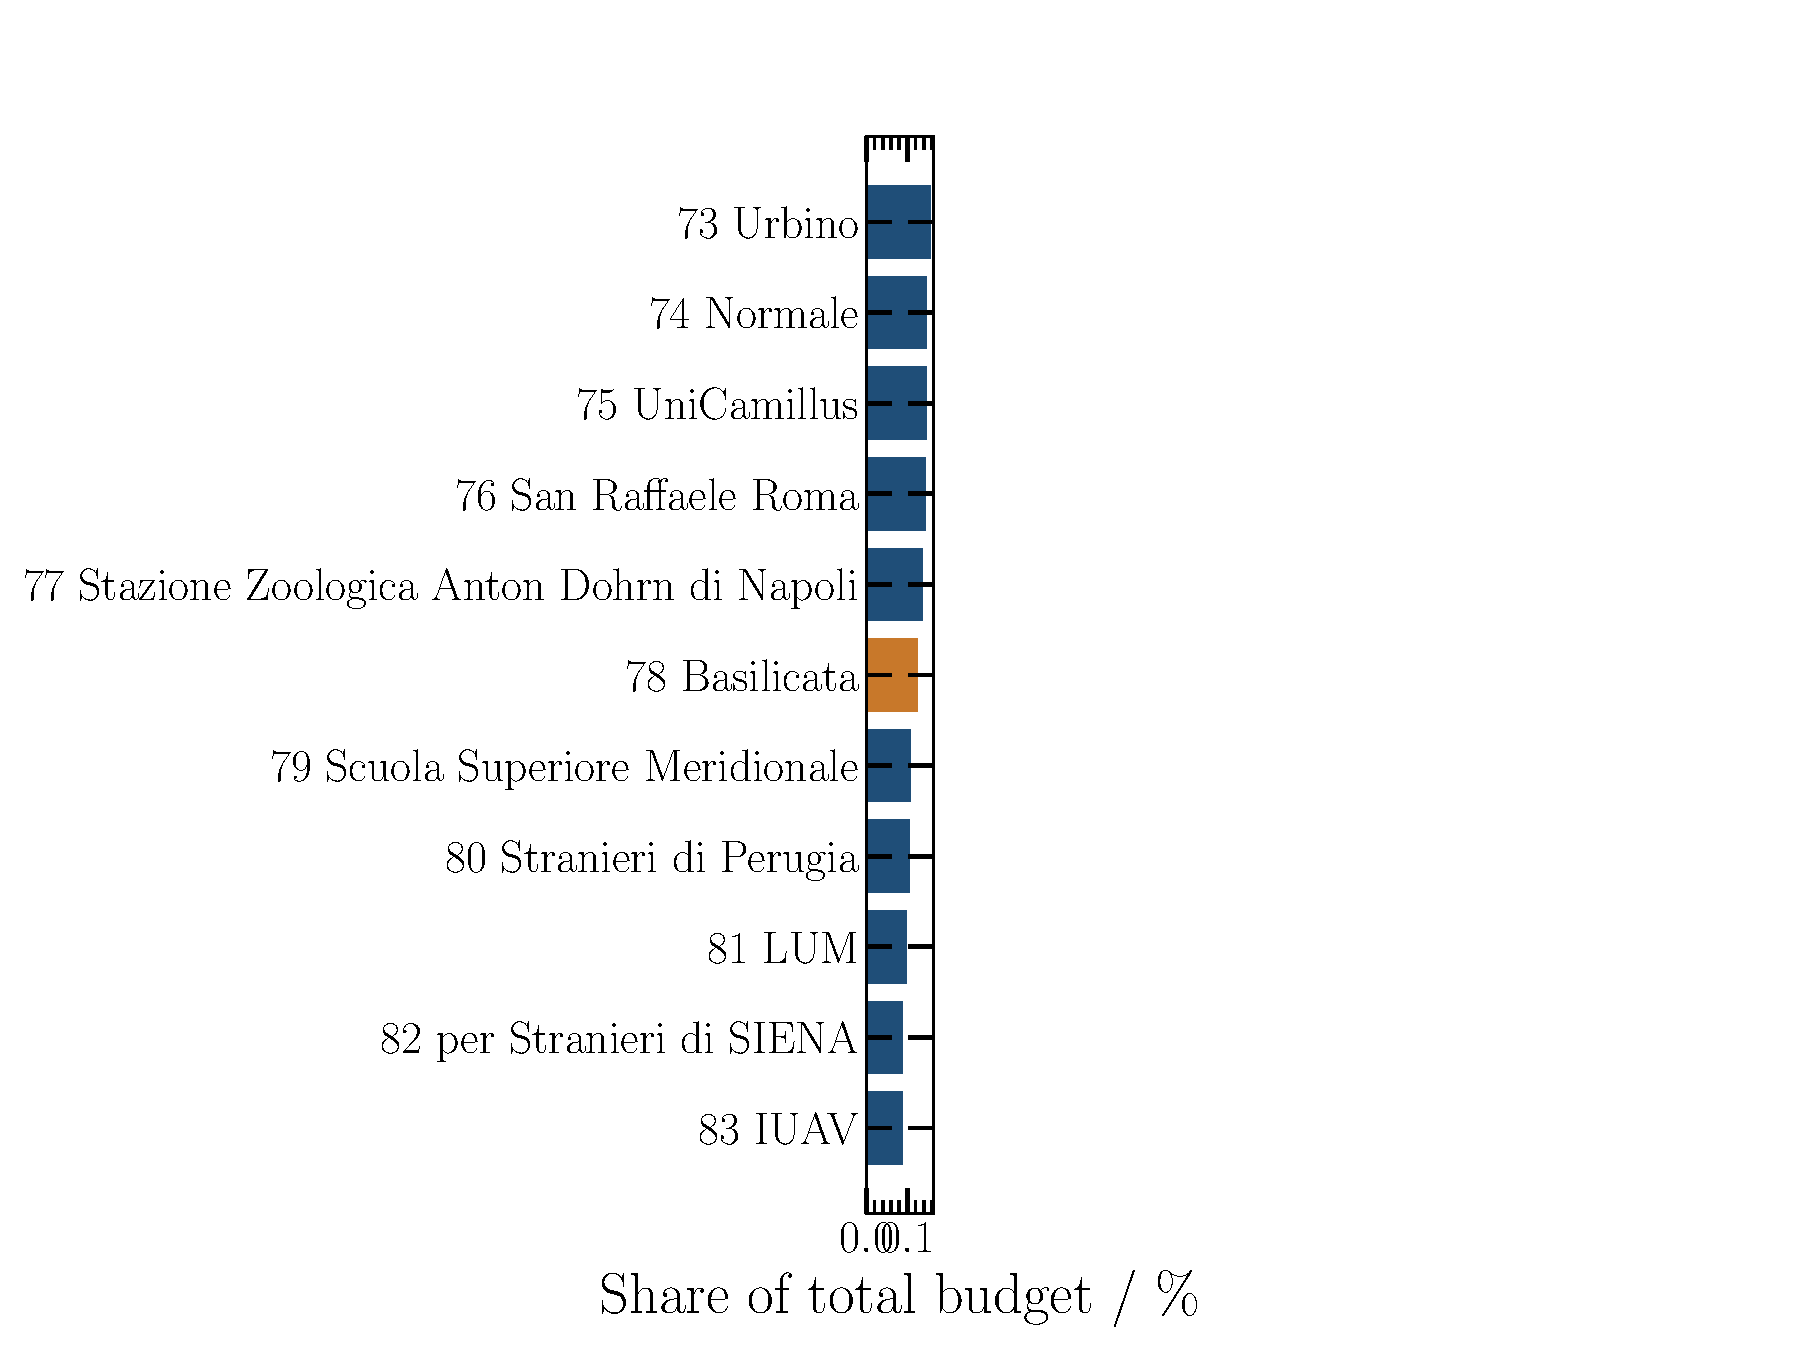
\includegraphics[width=0.65\textwidth]{../prin_out/figures/fact_basilicata_neighbours.pdf}
\caption{Share of the total budget of Basilicata and of the institutions ranked just above and below it.}
\end{figure}
\begin{figure}[H]
\centering
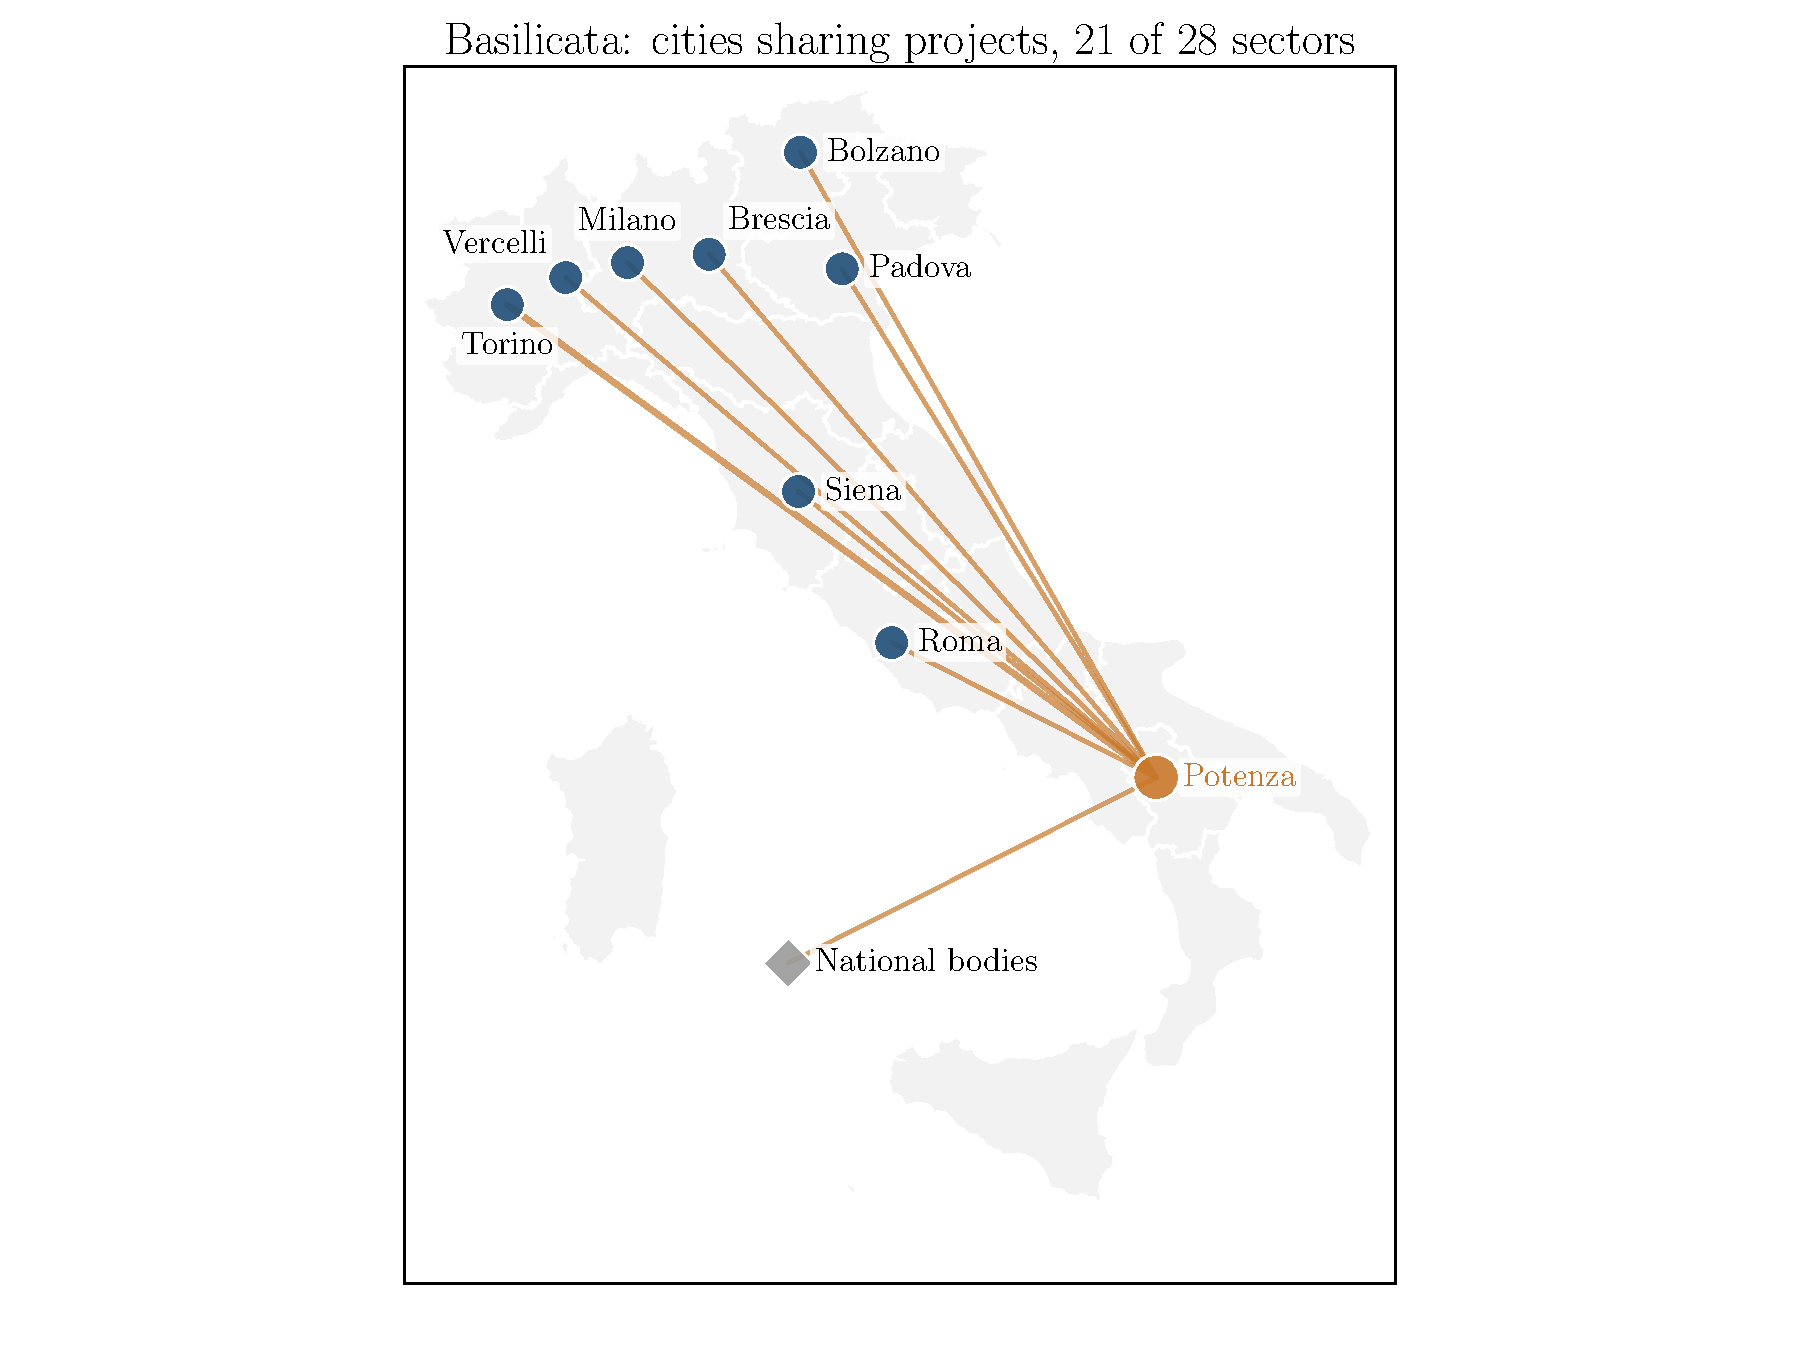
\includegraphics[width=0.75\textwidth]{../prin_out/figures/fact_basilicata_map.pdf}
\caption{Cities sharing funded projects with Basilicata (line width proportional to the number of projects).}
\end{figure}

\clearpage
\section{Institution fact sheet: Pisa}
\textbf{Purpose.} To collect the figures of one institution and compare them with the other institutions of the same type.

\textbf{Result.} Pisa received 5.37~M~EUR (2.49\% of the budget) in 25 projects, 4 as coordinator and 21 as partner, in 17 sectors; it ranks 10 of 91 institutions and 9 of 61 within its type.

\begin{table}[H]
\centering
\begin{tabular}{llr}
\toprule
Pisa & Value & Median, public univ. \\
\midrule
Funding & 5.37~M~EUR, 2.49\% of the budget & 0.76\% \\
Rank & 10 of 91; 9 of 61 in its type &  \\
Funded projects & 25 & 8 \\
Sectors with a funded unit & 17 of 24 & 7 \\
Money received as PI & 19\% & 21\% \\
\bottomrule
\end{tabular}
\end{table}
{\footnotesize
\begin{longtable}{lllrp{4.2cm}p{2cm}p{3.2cm}}
\toprule
Sector & Role & Level & k EUR & Project & Coordinator & Other institutions \\
\midrule
\endhead
LS3 & RU & PO & 302 & LIpid droplet COmmunication Networks In Cancer (LICONIC) & Padova & Perugia, Tor Vergata \\
LS4 & RU & PO & 160 & Diabetes-specific disruptors of cardiovascular resilience... & Padova & Humanitas University, Milano Statale, Sapienza, Tor Vergata \\
LS4 & RU & PA & 167 & PRISM-T2D BCAA-Klotho-FGF23 Axis as a Multidirectional... & Milano-Bicocca & Campus Bio-Medico, Sapienza, Torino, Vita-Salute San Raffaele \\
LS5 & RU & n.a. & 300 & RETRO-ALS: Endogenous retroelements as a lifespan axis of... & Sassari & Milano Statale, Trento \\
LS5 & RU & n.a. & 229 & MAPS-PD - Microplastic Accumulation and Parkinson's Disease:... & CNR & Federico II, Politecnico di Torino, Sant'Anna \\
LS7 & RU & PA & 169 & RISK-IT: Risk Miscalibration as a Fundamental Mechanism of... & Torino & Cagliari, Sapienza \\
LS8 & RU & n.a. & 183 & ECHOES (Ecological Connectivity and Hierarchical... & Sapienza & Bologna, Normale, Pavia, Siena \\
PE1 & RU & PA & 178 & Universality and Renormalization in Random Fields, Singular... & Milano-Bicocca & Pavia, Roma Tre, SISSA, Sapienza \\
PE1 & RU & RTD & 214 & The interplay of geometry and topology in the study of... & Bologna & Sapienza, Torino \\
PE1 & RU & PO & 188 & Order and randomness in Hamiltonian dynamics and dispersive PDEs & SISSA & Milano Statale, Roma Tre, Sapienza, Tor Vergata \\
PE10 & RU & PO & 206 & Mélanges Across Scales: Revealing the Rheological... & Torino & CNR, Genova, Modena e Reggio Emilia \\
PE10 & PI & PA & 267 & The dawn of the Humboldt Current System: Paleogene origins,... & this institution & Camerino, Milano-Bicocca, Torino \\
PE11 & RU & PA & 225 & HEAT: Hierarchical Engineering of infrAred Thermo-optical... & Sapienza & CNR, Padova, Politecnico di Milano \\
PE2 & RU & PO & 219 & Non-perturbative dynamics of fundamental interactions from... & Roma Tre & INFN, Milano-Bicocca, Tor Vergata, Torino \\
PE4 & PI & n.a. & 223 & DREAM-AIR - Defining risk in the exposome era: AI–driven... & this institution & Bologna, Chieti-Pescara, Genova, Politecnico di Milano, Salerno \\
PE4 & RU & n.a. & 171 & PROcesses for green dimethyl Ether from sUstainable Sources... & Milano Statale & CNR, Politecnico di Milano, Salerno, Torino \\
PE7 & RU & PA & 168 & Lab-to-Cell approach for online monitoring, diagnostics,... & Bologna & Brescia, Cassino, INRiM, Perugia \\
PE8 & RU & PO & 205 & AI-PRAESIDIUM — agentic AI for Performance-based Robustness... & Federico II & Bologna, IUAV, Salerno, Tor Vergata \\
PE9 & RU & PA & 269 & ET-STAR: Einstein Telescope – Science and Technical Advanced... & GSSI & INAF, INFN \\
SH3 & RU & n.a. & 174 & UnIneq - Understanding Inequality through Literacy and Frames & Politecnica delle Marche & Palermo, Pavia, Roma Tre, Universitas MERCATORUM \\
SH6 & RU & PA & 231 & Credit Italies. Banking, Industry, and the Geography of... & Insubria & Catania, Firenze, Parma \\
SH6 & RU & PA & 193 & FIRST-SICILY: FIRST entrance, dispersal and adaptation of... & Palermo & Bologna, CNR, Modena e Reggio Emilia \\
SH6 & PI & RTD & 284 & LEGALITES. Legal Elites and Social Transformation in the... & this institution & Bologna, Padova, Roma Tre \\
SH7 & PI & PO & 240 & AURORA- Artificial Intelligence and Urban Reconfigurations:... & this institution & Catania, Federico II, Firenze, IULM, Sapienza \\
SH8 & RU & n.a. & 211 & R4USEFilm. Retrieving, Revealing, Revisiting and Remixing... & Udine & Bologna, Cagliari, Parma \\
\midrule
Total &  &  & 5374 &  &  &  \\
\bottomrule
\multicolumn{7}{l}{\footnotesize Level of the leader: PO, PA, RTD, RU; n.a.: not a university leader or not found.} \\
\end{longtable}
}
\begin{figure}[H]
\centering
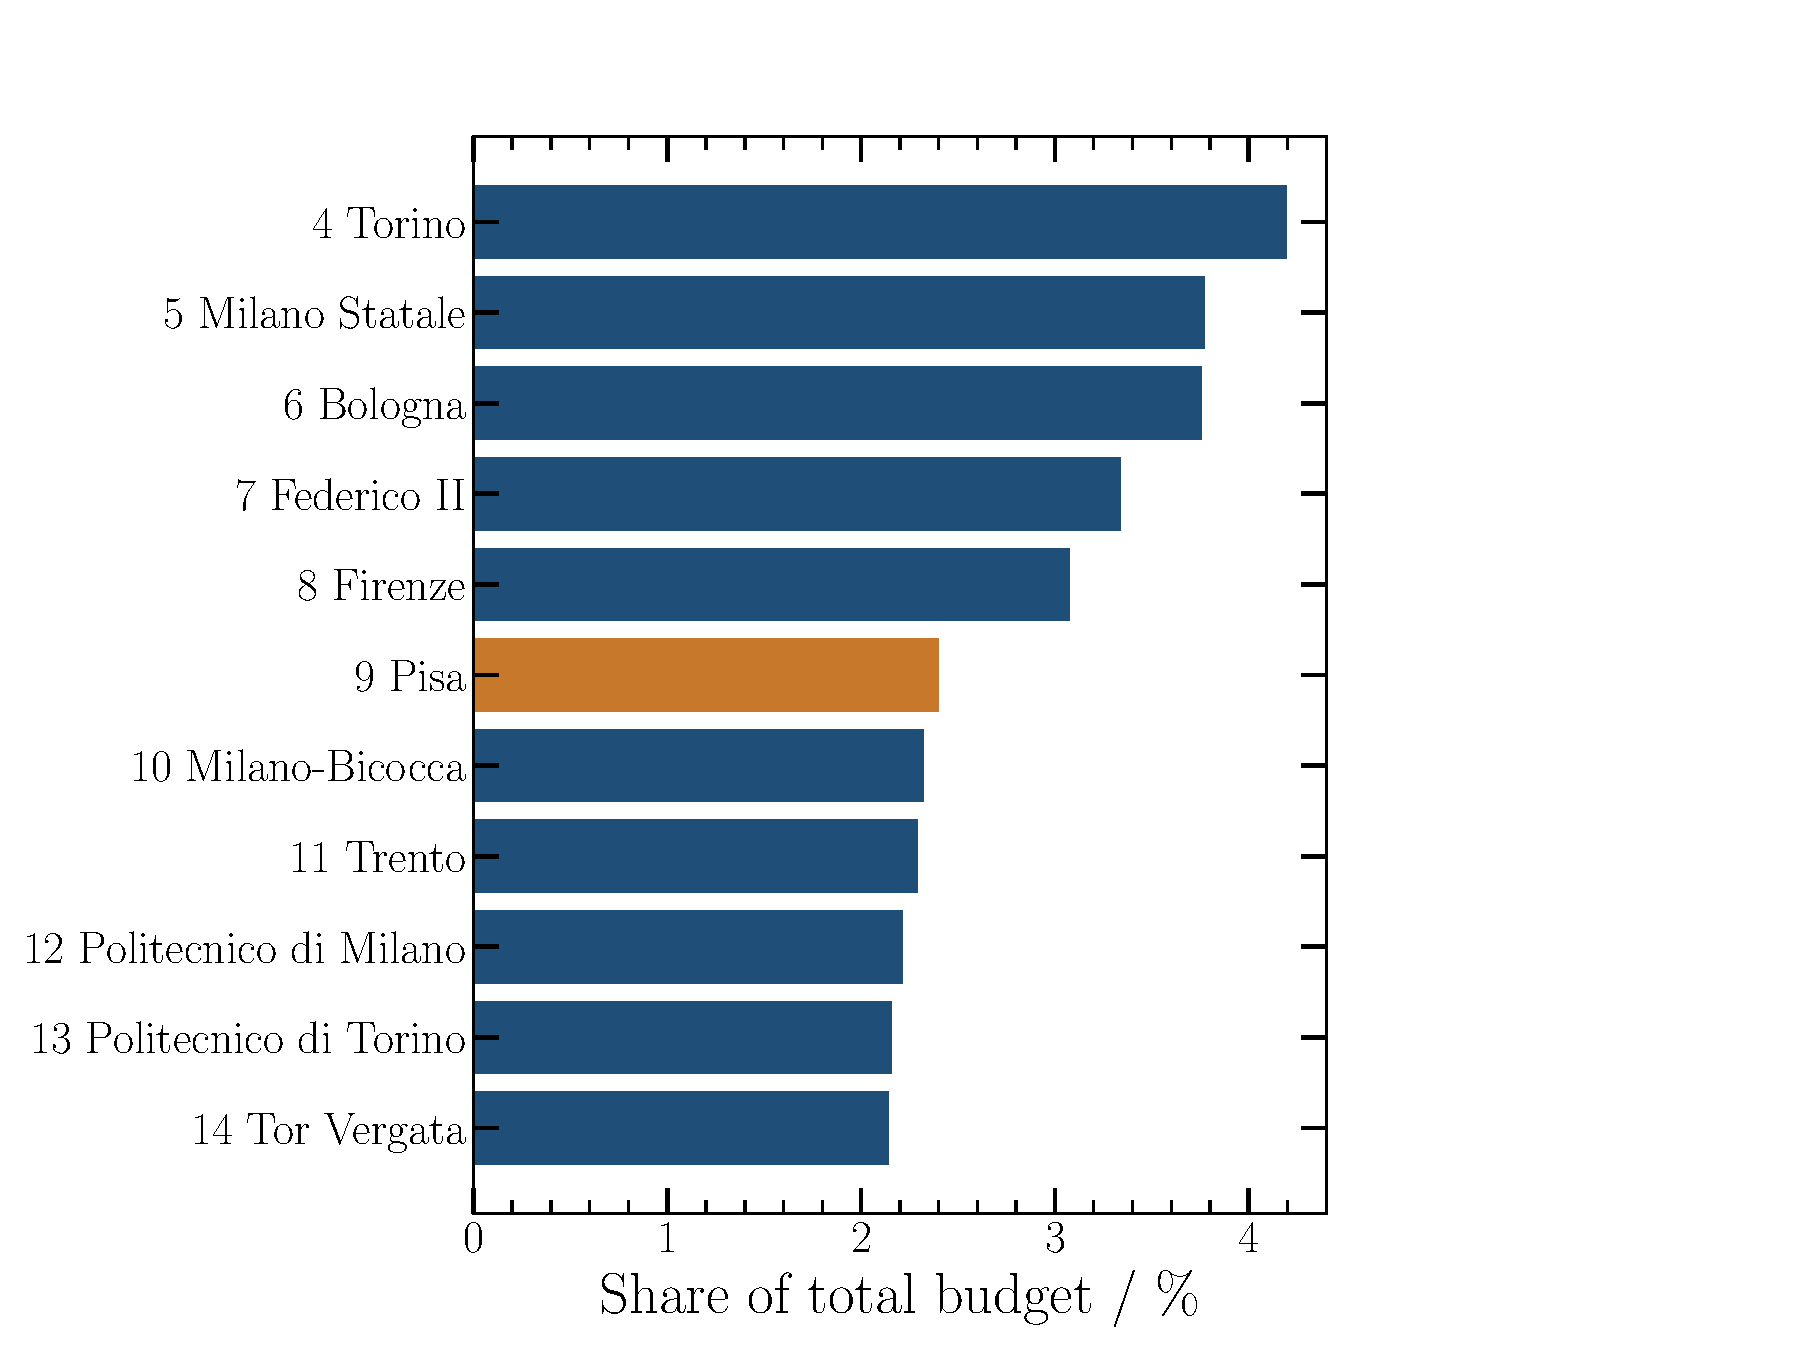
\includegraphics[width=0.65\textwidth]{../prin_out/figures/fact_pisa_neighbours.pdf}
\caption{Share of the total budget of Pisa and of the institutions ranked just above and below it.}
\end{figure}
\begin{figure}[H]
\centering
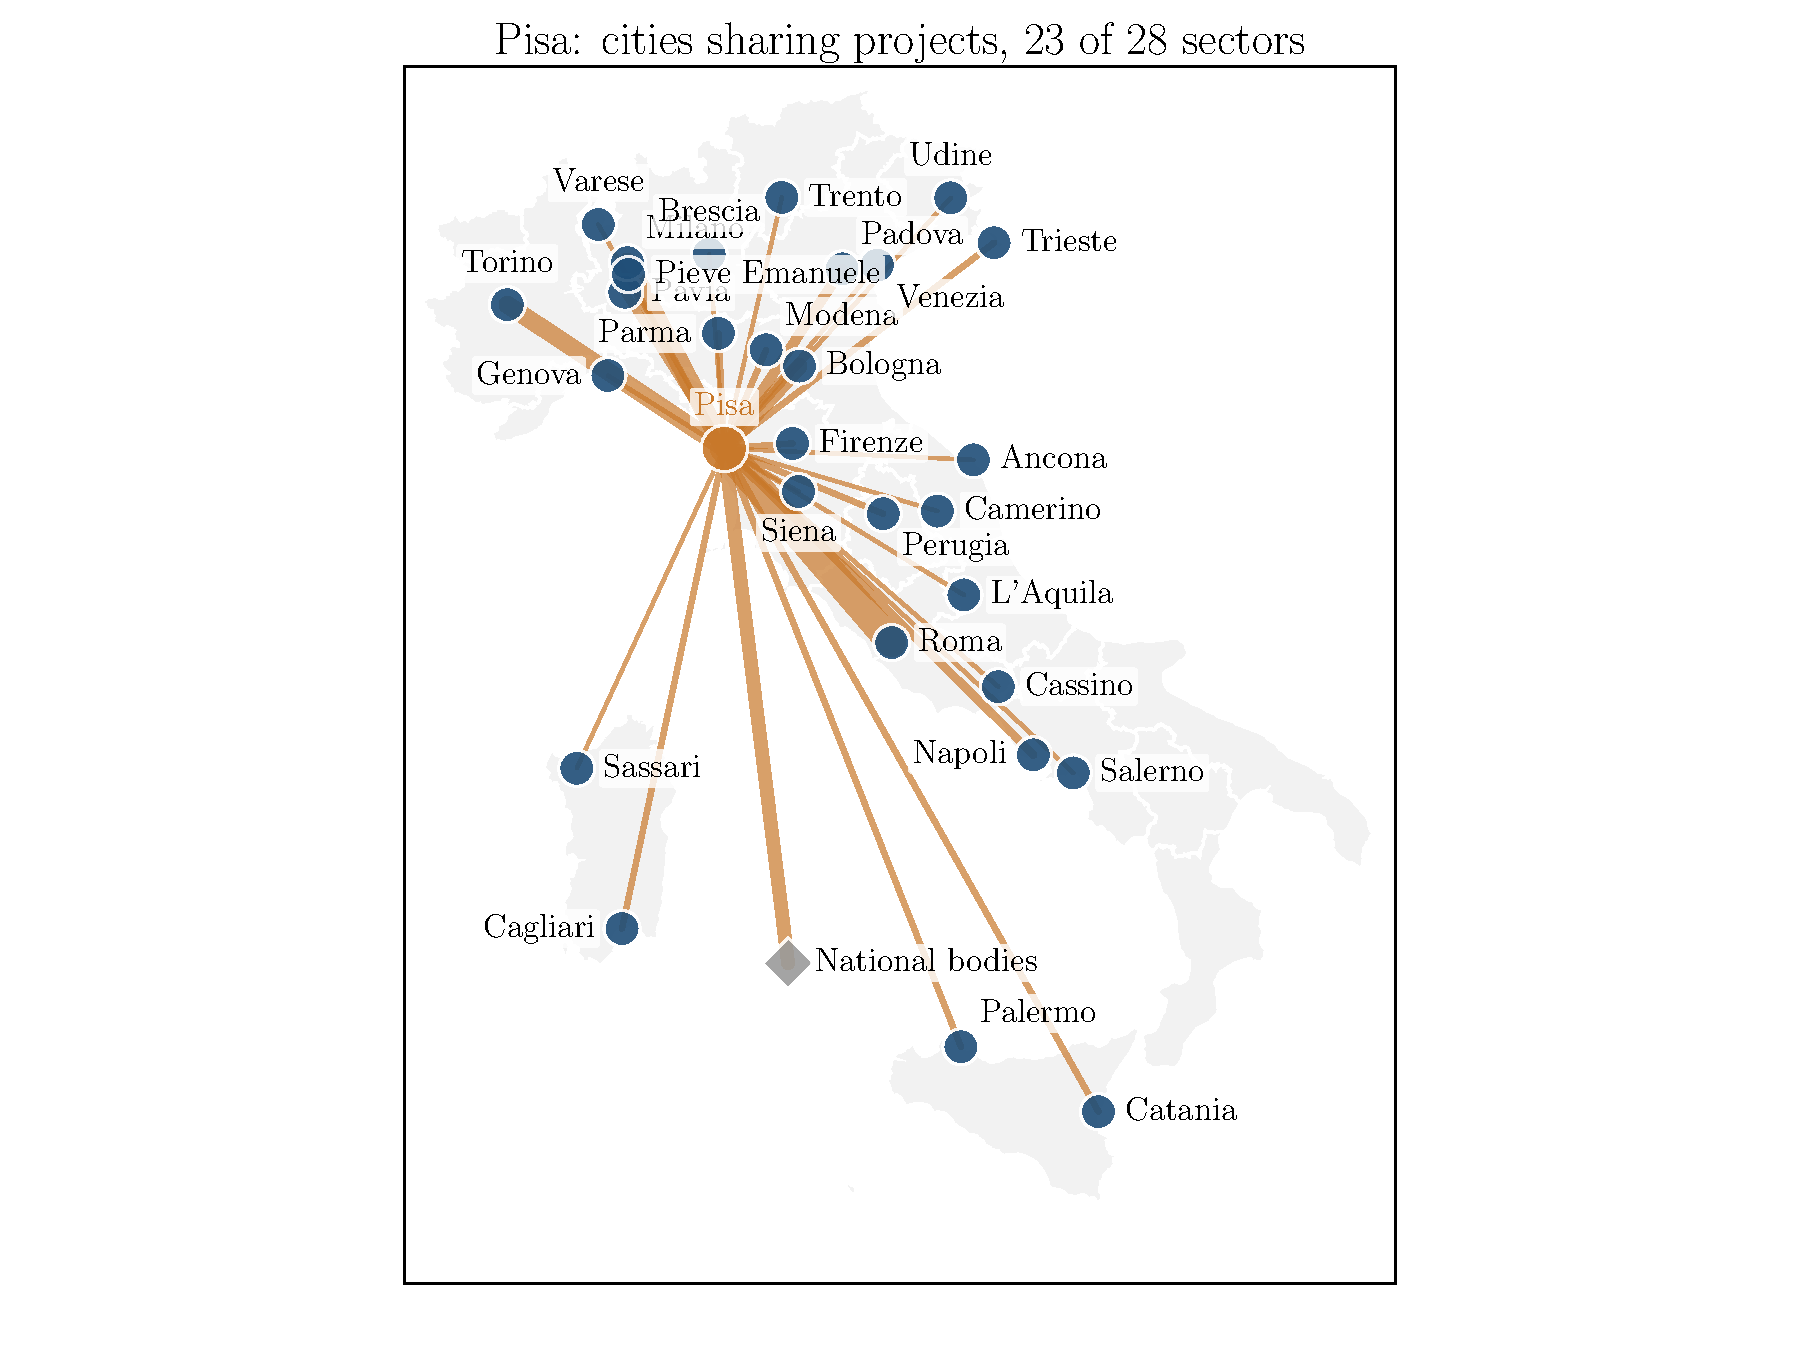
\includegraphics[width=0.75\textwidth]{../prin_out/figures/fact_pisa_map.pdf}
\caption{Cities sharing funded projects with Pisa (line width proportional to the number of projects).}
\end{figure}

\clearpage
\section{Institution fact sheet: Normale}
\textbf{Purpose.} To collect the figures of one institution and compare them with the other institutions of the same type.

\textbf{Result.} Normale received 0.34~M~EUR (0.16\% of the budget) in 2 projects, 1 as coordinator and 1 as partner, in 2 sectors; it ranks 74 of 91 institutions and 6 of 7 within its type.

\begin{table}[H]
\centering
\begin{tabular}{llr}
\toprule
Normale & Value & Median, advanced schools \\
\midrule
Funding & 0.34~M~EUR, 0.16\% of the budget & 0.33\% \\
Rank & 74 of 91; 6 of 7 in its type &  \\
Funded projects & 2 & 3 \\
Sectors with a funded unit & 2 of 24 & 2 \\
Money received as PI & 63\% & 44\% \\
\bottomrule
\end{tabular}
\end{table}
{\footnotesize
\begin{longtable}{lllrp{4.2cm}p{2cm}p{3.2cm}}
\toprule
Sector & Role & Level & k EUR & Project & Coordinator & Other institutions \\
\midrule
\endhead
LS8 & RU & n.a. & 126 & ECHOES (Ecological Connectivity and Hierarchical... & Sapienza & Bologna, Pavia, Pisa, Siena \\
PE1 & PI & PO & 211 & Variational Methods, Geometric Analysis and Free Boundary... & this institution & Politecnico di Milano, Sapienza, Tor Vergata, Torino, Trento \\
\midrule
Total &  &  & 338 &  &  &  \\
\bottomrule
\multicolumn{7}{l}{\footnotesize Level of the leader: PO, PA, RTD, RU; n.a.: not a university leader or not found.} \\
\end{longtable}
}
\begin{figure}[H]
\centering
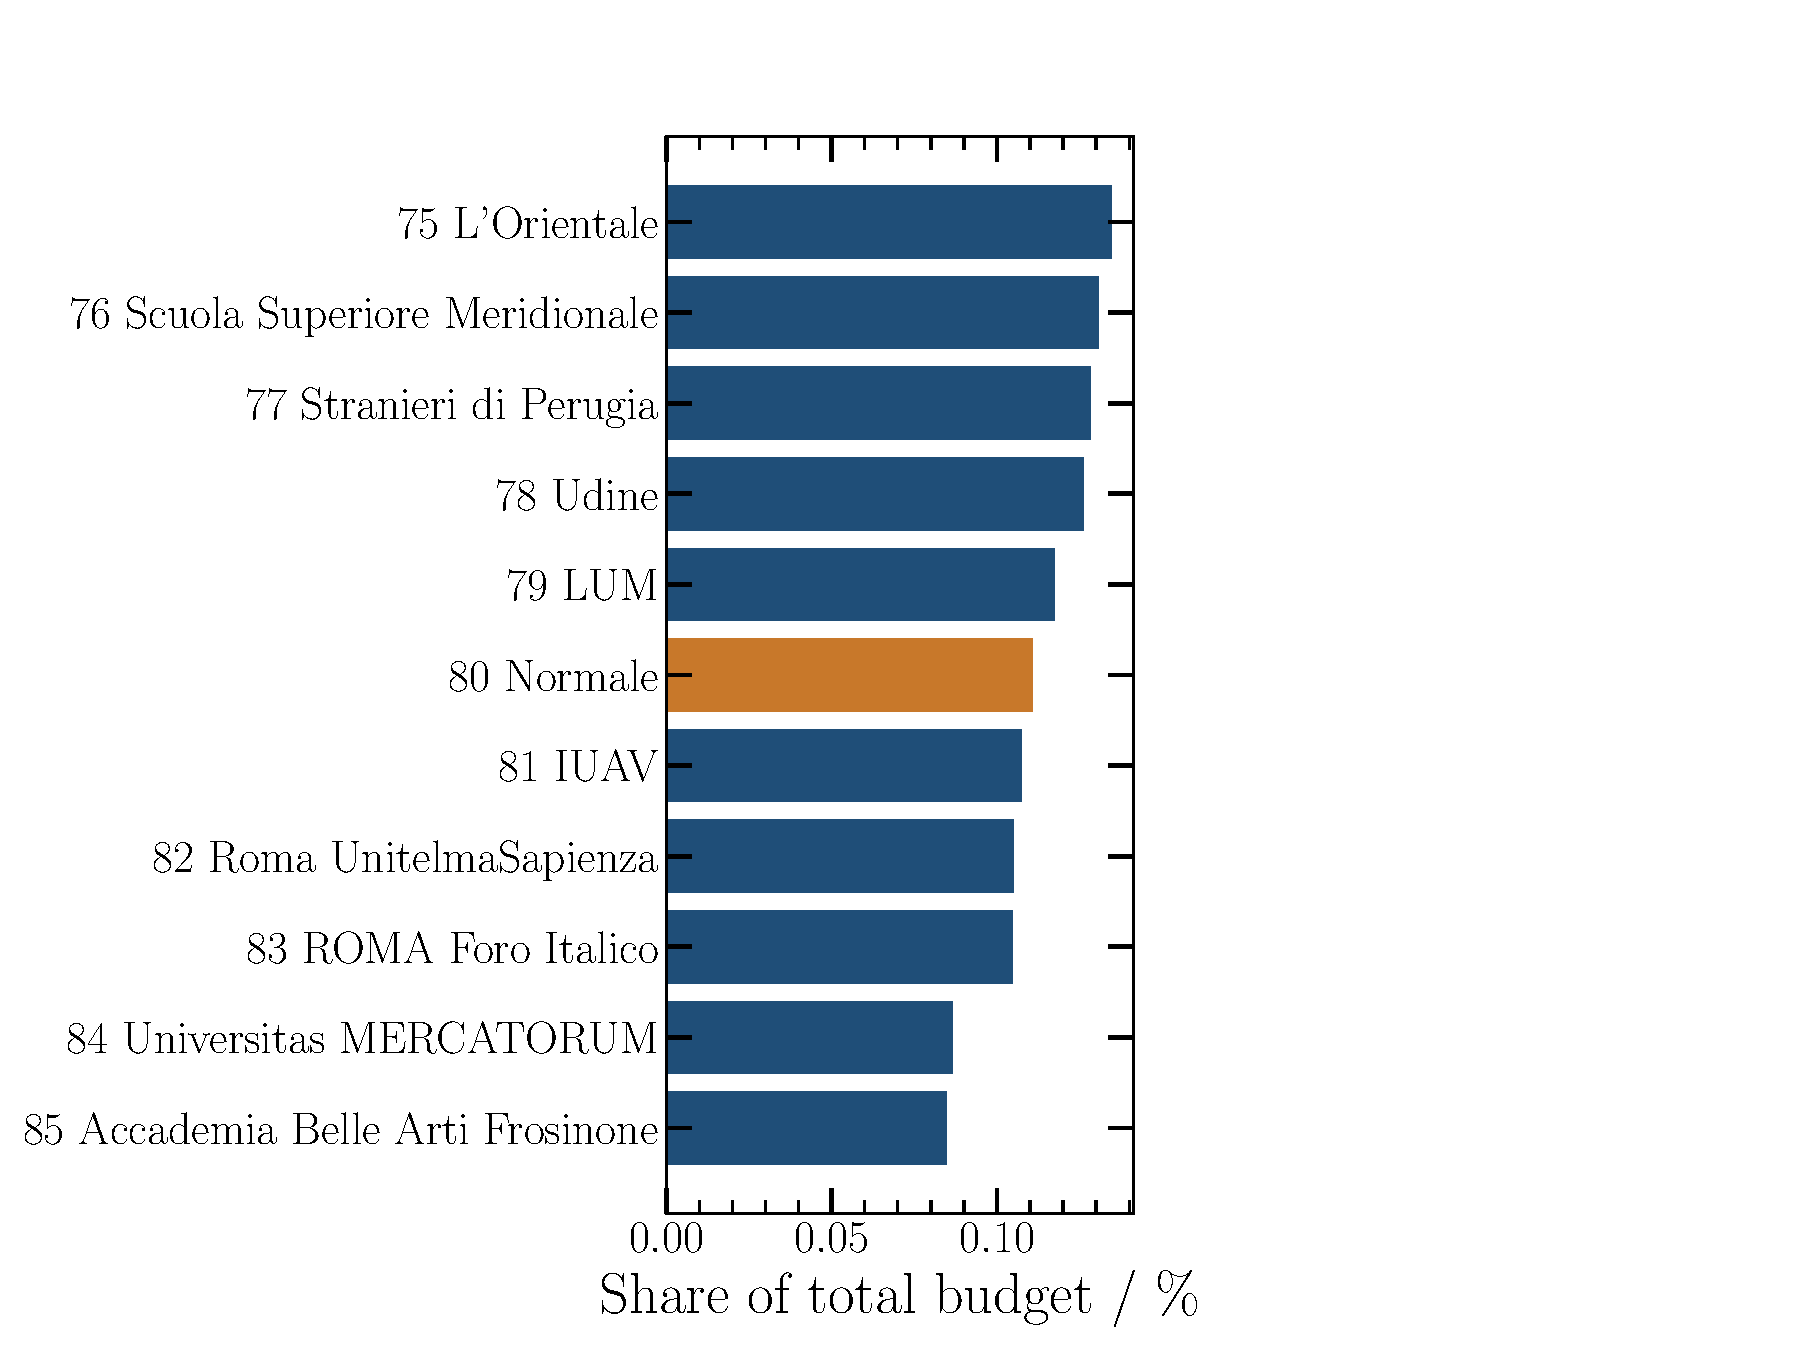
\includegraphics[width=0.65\textwidth]{../prin_out/figures/fact_normale_neighbours.pdf}
\caption{Share of the total budget of Normale and of the institutions ranked just above and below it.}
\end{figure}
\begin{figure}[H]
\centering
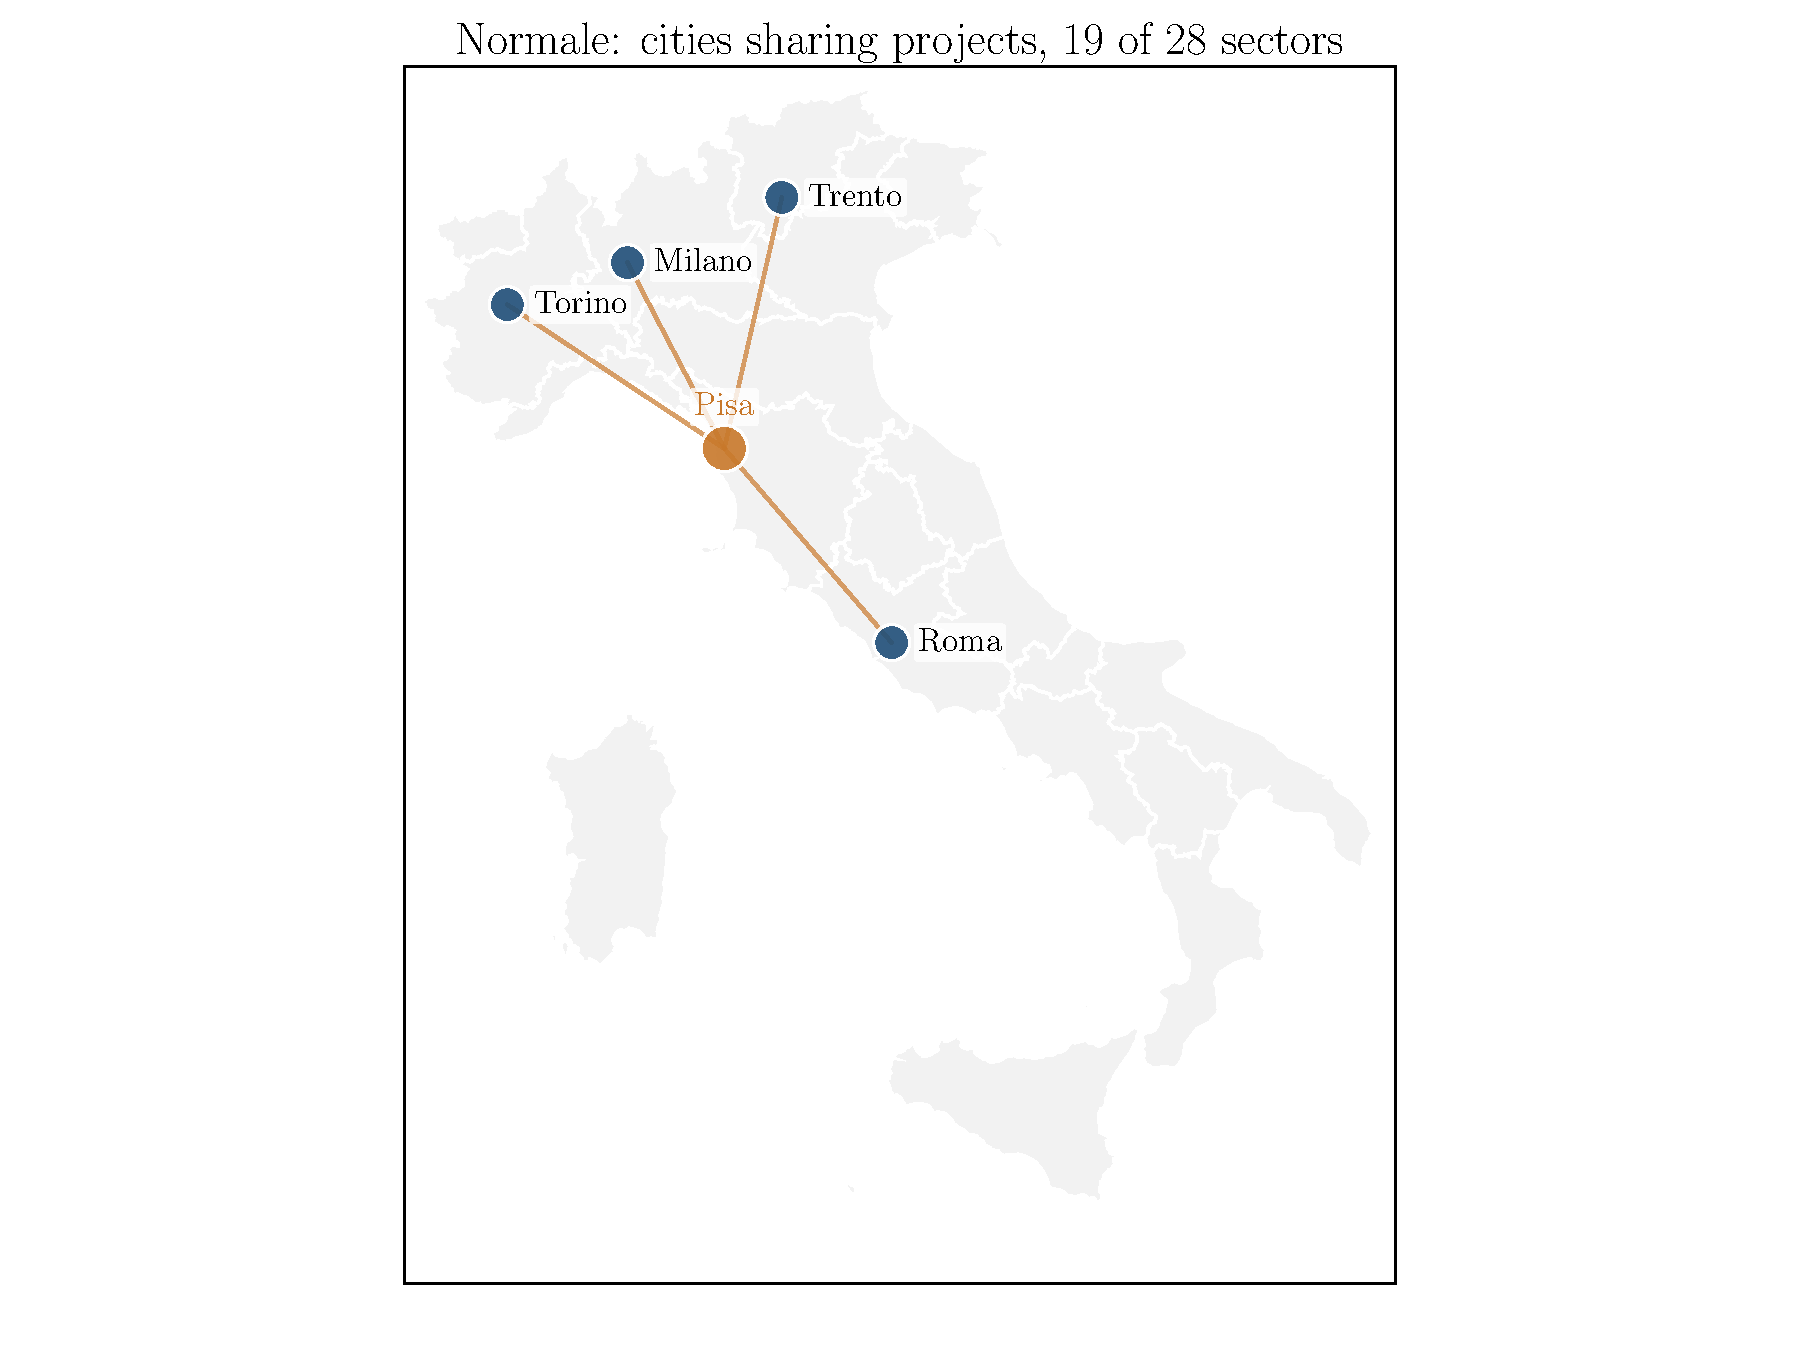
\includegraphics[width=0.75\textwidth]{../prin_out/figures/fact_normale_map.pdf}
\caption{Cities sharing funded projects with Normale (line width proportional to the number of projects).}
\end{figure}

\clearpage
\section{Institution fact sheet: Padova}
\textbf{Purpose.} To collect the figures of one institution and compare them with the other institutions of the same type.

\textbf{Result.} Padova received 9.24~M~EUR (4.29\% of the budget) in 41 projects, 14 as coordinator and 27 as partner, in 18 sectors; it ranks 4 of 91 institutions and 3 of 61 within its type.

\begin{table}[H]
\centering
\begin{tabular}{llr}
\toprule
Padova & Value & Median, public univ. \\
\midrule
Funding & 9.24~M~EUR, 4.29\% of the budget & 0.76\% \\
Rank & 4 of 91; 3 of 61 in its type &  \\
Funded projects & 41 & 8 \\
Sectors with a funded unit & 18 of 24 & 7 \\
Money received as PI & 41\% & 21\% \\
\bottomrule
\end{tabular}
\end{table}
{\footnotesize
\begin{longtable}{lllrp{4.2cm}p{2cm}p{3.2cm}}
\toprule
Sector & Role & Level & k EUR & Project & Coordinator & Other institutions \\
\midrule
\endhead
LS2 & PI & PO & 335 & Leveraging multidisciplinary expertise to identify new... & this institution & Modena e Reggio Emilia, Perugia, Sapienza \\
LS2 & PI & RTD & 318 & Deciphering how conformational landscape converts... & this institution & L'Aquila, Milano Statale, Sapienza \\
LS3 & PI & PO & 323 & LIpid droplet COmmunication Networks In Cancer (LICONIC) & this institution & Perugia, Pisa, Tor Vergata \\
LS3 & PI & PO & 302 & Multiscale dissection of Collagen VI landscapes in... & this institution & Bologna, CNR, Campus Bio-Medico, Tor Vergata \\
LS3 & RU & PO & 240 & Dynamic interplay between cell-intrinsic and cell-extrinsic... & Trieste & CNR, Milano Statale, Politecnico di Milano \\
LS3 & RU & PO & 301 & The conventional and unconventional roles of the... & Milano Statale & Bologna, Torino \\
LS4 & PI & PO & 185 & Diabetes-specific disruptors of cardiovascular resilience... & this institution & Humanitas University, Milano Statale, Pisa, Sapienza, Tor Vergata \\
LS7 & RU & PA & 196 & MIND-AGE: Molecular mechanisms of accelerated agINg in mood... & Cagliari & Brescia, Foggia, Teramo \\
LS7 & RU & PA & 226 & ADVANCES — AAV host factor Discovery, VAlidation, and... & Pavia & CNR, Vanvitelli \\
LS8 & RU & n.a. & 169 & CHEMO-EMO - Chemical Signals of Emotion: Bridging Humans,... & Federico II & CNR, Firenze \\
LS8 & RU & n.a. & 195 & RESPOND - Integrated ecological and evolutionary responses... & Milano Statale & Torino, Tuscia \\
LS8 & PI & n.a. & 440 & TRANSMIT: Towards a mechanistic and predictive framework of... & this institution & Bologna, Federico II, Sapienza \\
LS8 & PI & n.a. & 328 & NOVel Artificial MARine Ecosystems: linking behaviour,... & this institution & Firenze, Palermo, Politecnica delle Marche \\
PE10 & PI & PO & 235 & A Multidisciplinary AppROach to unravel the seismic cycle in... & this institution & Federico II, INGV, Milano-Bicocca, Torino \\
PE10 & RU & PO & 172 & Eocene Thermal optimum with EC-Earth4: proxy Reconstruction... & Politecnico di Torino & CNR, INGV, Urbino \\
PE10 & RU & RTD & 117 & REACT - Rapid rEsponse to Alpine Climatological Threats for... & Firenze & Bologna, CNR, INGV, Politecnico di Torino \\
PE11 & RU & PO & 128 & HEAT: Hierarchical Engineering of infrAred Thermo-optical... & Sapienza & CNR, Pisa, Politecnico di Milano \\
PE2 & PI & PA & 256 & Collider Pathways to New Physics in the Precision Era & this institution & Bologna, INFN, Sapienza \\
PE3 & RU & PO & 186 & Equilibrium and Non-Equilibrium Transport in complex GELS:... & CNR & Firenze, Milano Statale, Sapienza \\
PE3 & RU & PA & 170 & PROTEUS: Physics of Cancer Dynamics: Single Cells,... & Milano Statale & Sapienza, Torino, Vita-Salute San Raffaele \\
PE5 & PI & PO & 173 & TWIST — ToWard chiral light from Inverted Singlet-Triplet... & this institution & Basilicata, Bolzano, Brescia, Siena, Torino \\
PE5 & RU & PO & 191 & SPIRAL: Chirality-Driven SPIN Control of Photocatalytic... & Salento & Firenze, Magna Graecia, Modena e Reggio Emilia, Perugia \\
PE5 & RU & PA & 176 & FLUOride TRAPping through bridged dimeric metal complexes: A... & Piemonte Orientale & Modena e Reggio Emilia, Palermo, Parma \\
PE5 & RU & PO & 173 & Spatially Programmed 3D Adsorbents for Carbon dioxidE... & Torino & CNR, Milano Statale, Milano-Bicocca, Perugia \\
PE5 & PI & PA & 199 & Cross-coupling strategies for the sustainable synthesis of... & this institution & Bari Aldo Moro, Genova, Milano Statale, Pavia, Tuscia \\
PE6 & RU & PA & 170 & Embodied eXPERtise Transfer through Mutual Interpretation... & Verona & Bolzano, Catania, Federico II, Sapienza \\
PE7 & RU & PO & 197 & Photonic Highways for Advanced Real-time Observation and... & L'Aquila & Parma, Politecnico di Milano, Politecnico di Torino \\
PE7 & RU & PA & 176 & Metrological framework for TRUSTworthy MEasuring systems... & Firenze & Cassino, Cattolica, Salerno, Trento \\
PE7 & RU & PO & 262 & DENDRA - Adaptive Dendritic Electronics for Self-Organizing... & Torino & CNR, Tor Vergata \\
PE8 & RU & PO & 240 & LACES – Low-impact Advanced Concrete Engineering Systems:... & Trento & Federico II, Modena e Reggio Emilia, Perugia \\
PE8 & RU & PA & 211 & AURA - Atmospheric hUmidity Recovery with Advanced sorbents & CNR & Messina, Politecnico di Milano, Politecnico di Torino \\
PE8 & RU & RTD & 199 & ENCHANT – ENgineered Co-design of surfaces and geometries... & Parma & Bologna, Firenze, Pavia, Politecnico di Milano \\
PE9 & RU & RTD & 165 & Augmented Physics for EXtremes (APEX) & INAF & Bologna, Cagliari, Politecnico di Milano \\
SH3 & RU & n.a. & 270 & FLUENCE – Processing FLUency and Political InfluENCE & Milano-Bicocca & Modena e Reggio Emilia, Pavia \\
SH3 & PI & n.a. & 315 & COBIKE - Co-Making Urban Cycling Infrastructures:... & this institution & CNR, Siena, Torino \\
SH4 & RU & PO & 240 & The Multimodal Turn: Uncovering the Neurocognitive... & Trento & IMT Lucca, SISSA \\
SH5 & PI & RTD & 220 & TRACE – Text and Reception of the Aristotelian Corpus: The... & this institution & Bari Aldo Moro, Federico II, Macerata, Messina, Sapienza \\
SH5 & RU & n.a. & 185 & What’s the Matter? Matter as an Epistemic and Ontological... & Catania & Bari Aldo Moro, Messina, Pavia, Salento \\
SH6 & RU & RTD & 219 & AFTER: Afterlives of fascism in everyday spaces & Siena & L'Aquila, Torino, Trento \\
SH6 & PI & PA & 193 & HERB-IT Herbaria as Knowledge Infrastructures: Shaping... & this institution & Catania, Ferrara, Firenze, Insubria, Sapienza \\
SH6 & RU & PA & 244 & LEGALITES. Legal Elites and Social Transformation in the... & Pisa & Bologna, Roma Tre \\
\midrule
Total &  &  & 9237 &  &  &  \\
\bottomrule
\multicolumn{7}{l}{\footnotesize Level of the leader: PO, PA, RTD, RU; n.a.: not a university leader or not found.} \\
\end{longtable}
}
\begin{figure}[H]
\centering
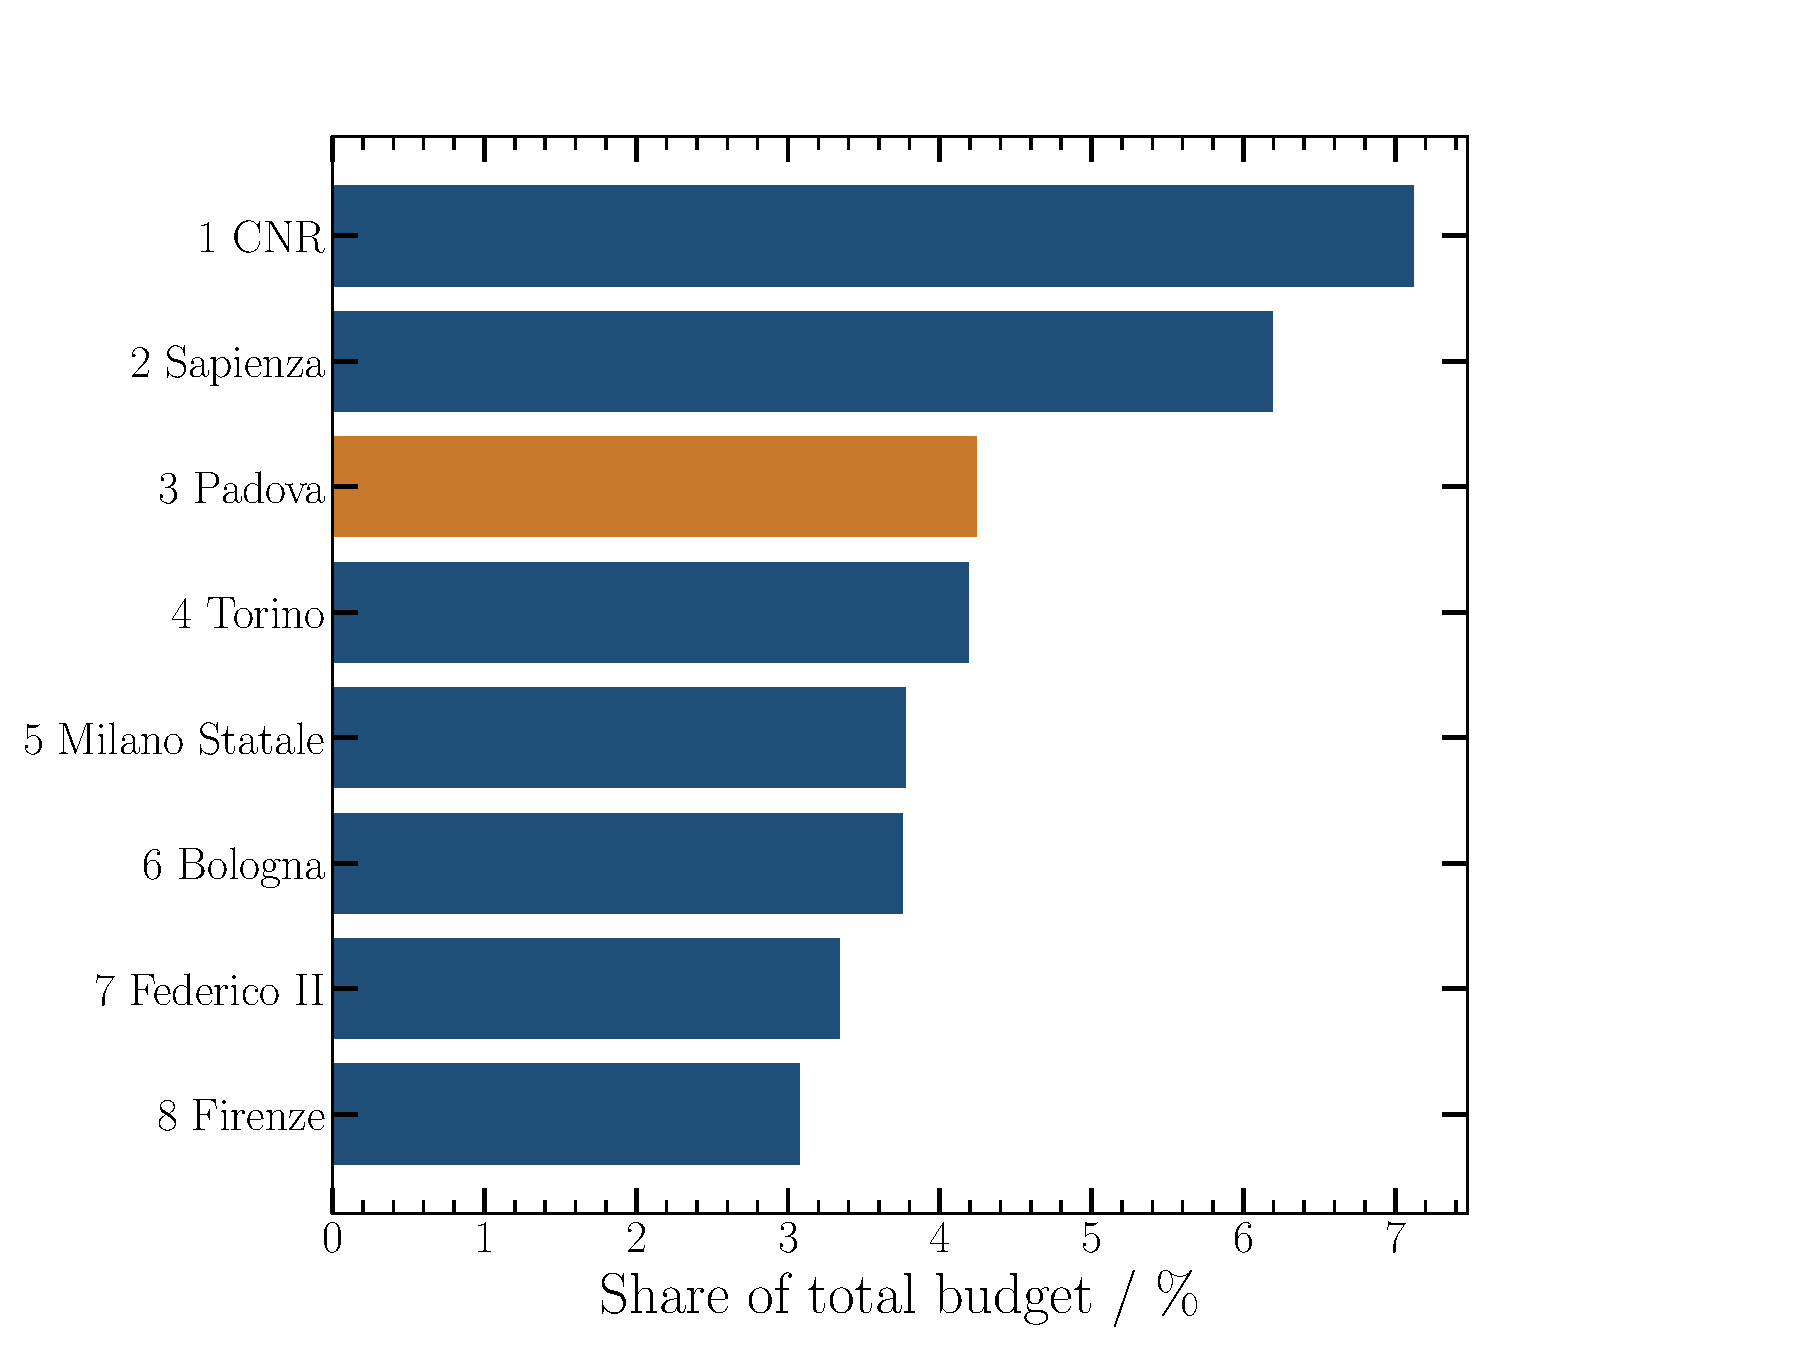
\includegraphics[width=0.65\textwidth]{../prin_out/figures/fact_padova_neighbours.pdf}
\caption{Share of the total budget of Padova and of the institutions ranked just above and below it.}
\end{figure}
\begin{figure}[H]
\centering
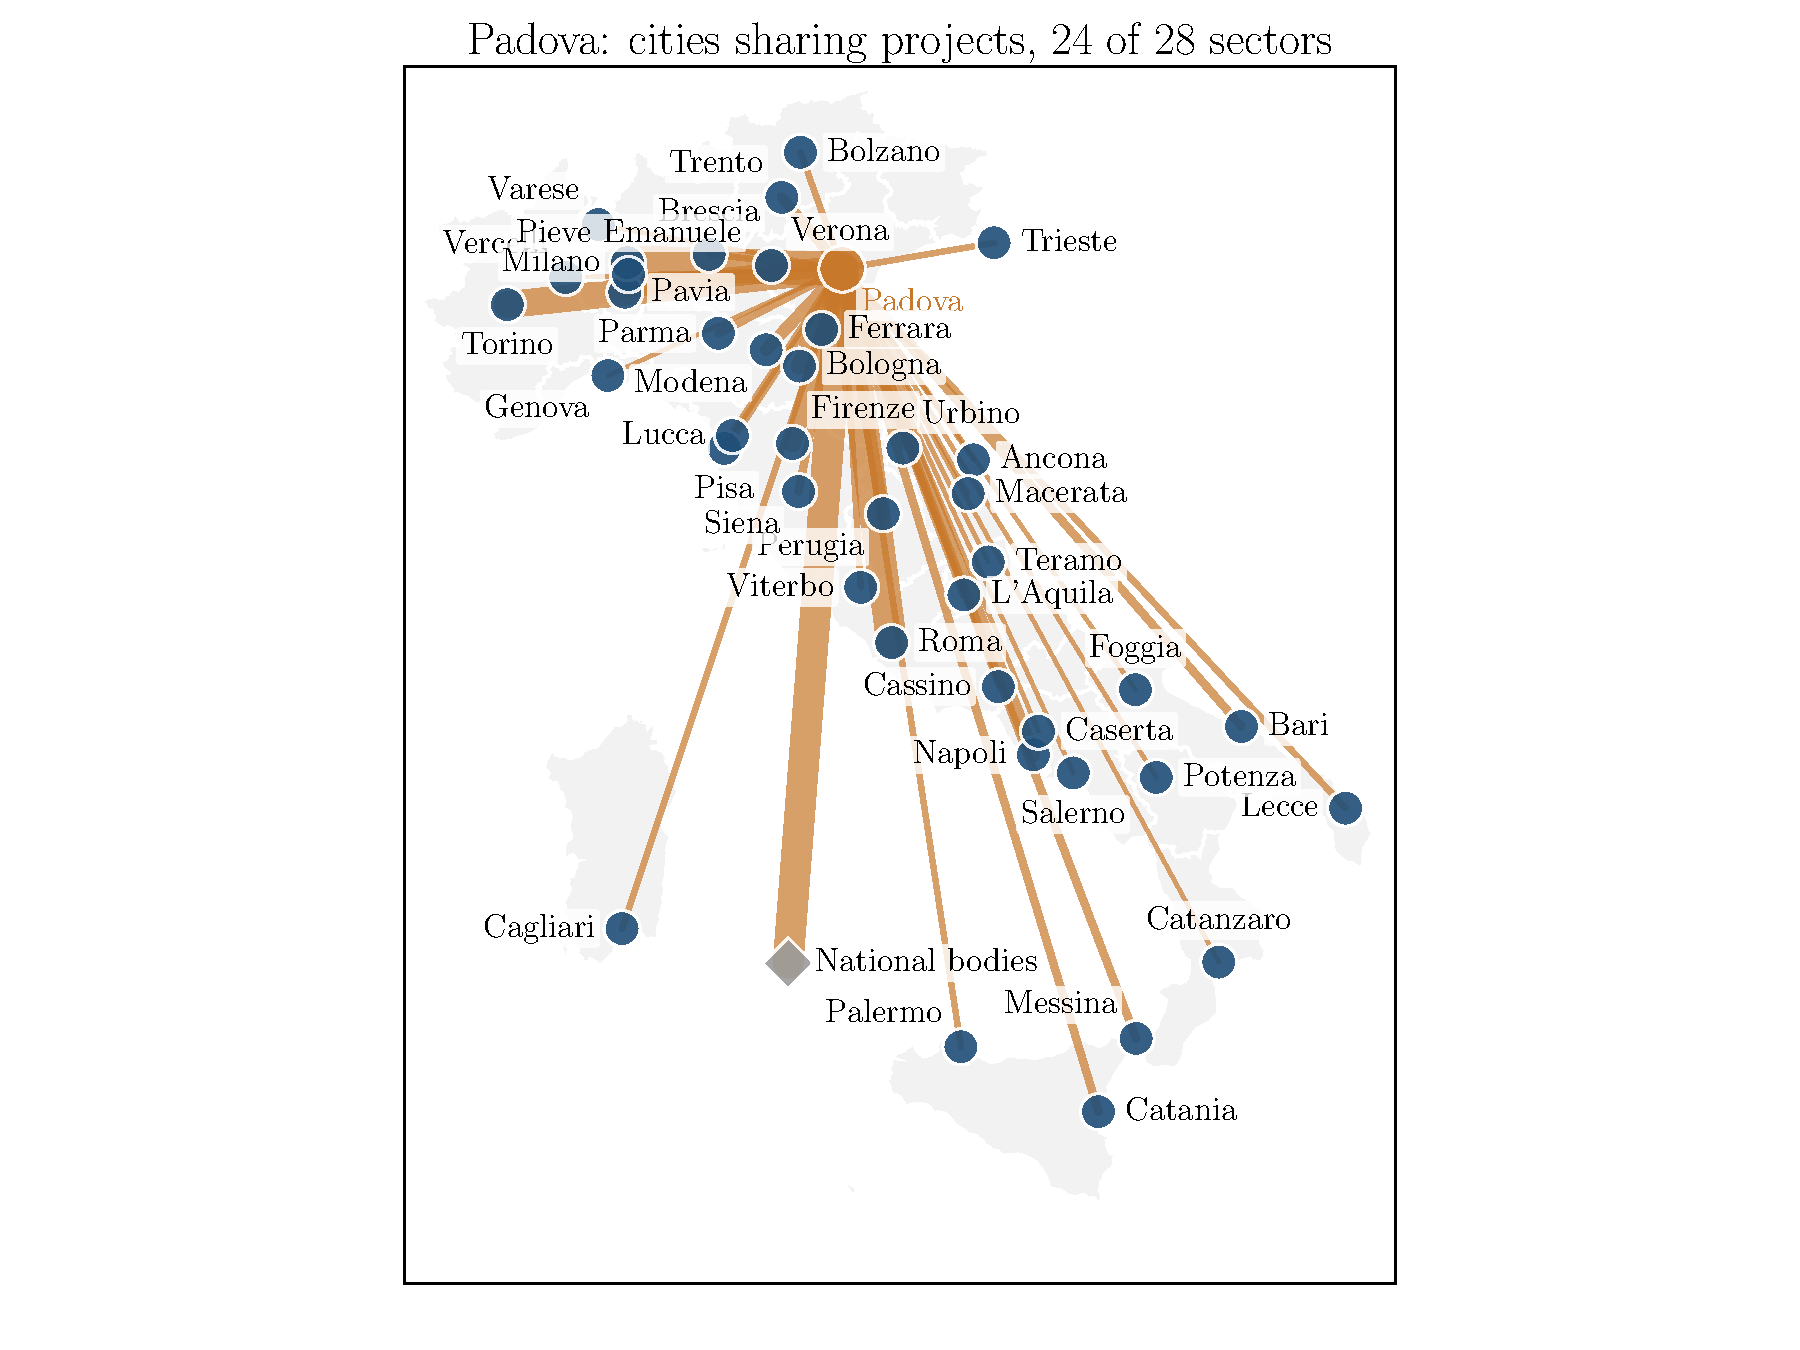
\includegraphics[width=0.75\textwidth]{../prin_out/figures/fact_padova_map.pdf}
\caption{Cities sharing funded projects with Padova (line width proportional to the number of projects).}
\end{figure}

\clearpage
\section{Institution fact sheet: Brescia}
\textbf{Purpose.} To collect the figures of one institution and compare them with the other institutions of the same type.

\textbf{Result.} Brescia received 1.92~M~EUR (0.89\% of the budget) in 10 projects, 1 as coordinator and 9 as partner, in 7 sectors; it ranks 30 of 91 institutions and 28 of 61 within its type.

\begin{table}[H]
\centering
\begin{tabular}{llr}
\toprule
Brescia & Value & Median, public univ. \\
\midrule
Funding & 1.92~M~EUR, 0.89\% of the budget & 0.76\% \\
Rank & 30 of 91; 28 of 61 in its type &  \\
Funded projects & 10 & 8 \\
Sectors with a funded unit & 7 of 24 & 7 \\
Money received as PI & 12\% & 21\% \\
\bottomrule
\end{tabular}
\end{table}
{\footnotesize
\begin{longtable}{lllrp{4.2cm}p{2cm}p{3.2cm}}
\toprule
Sector & Role & Level & k EUR & Project & Coordinator & Other institutions \\
\midrule
\endhead
LS2 & RU & PO & 202 & Decoding and Targeting Cancer Plasticity & Vita-Salute San Raffaele & Palermo, Torino, Trento \\
LS4 & RU & PA & 164 & Decoding the Multi-Organ Interfaces Driving Adaptive or... & Sapienza & Bologna, Humanitas University, Insubria, Milano Statale \\
LS6 & RU & PA & 216 & The self-reactive root: how BCR autoreactivity shapes... & Milano Statale & CNR, Cattolica, Vita-Salute San Raffaele \\
LS6 & PI & PO & 233 & INTEGRATIVE DISSECTION AND GENE CORRECTION OF IMMUNE... & this institution & Federico II, Firenze, Sapienza, Verona \\
LS7 & RU & PA & 197 & MIND-AGE: Molecular mechanisms of accelerated agINg in mood... & Cagliari & Foggia, Padova, Teramo \\
LS7 & RU & PO & 203 & Postbiotic-Mediated Reprogramming of Inflammatory,... & Catania & Calabria, Federico II, Sapienza, Vanvitelli \\
PE2 & RU & PA & 165 & Ultracold MOlecules in Arrays of optical Traps (U-MOAT) & CNR & Firenze, INRiM \\
PE5 & RU & PA & 173 & TWIST — ToWard chiral light from Inverted Singlet-Triplet... & Padova & Basilicata, Bolzano, Siena, Torino \\
PE7 & RU & PA & 222 & e-DoIT-RISE - echo-Doppler Imaging Tonometer: Reference... & Roma Tre & Catania, Unicusano \\
PE7 & RU & PO & 140 & Lab-to-Cell approach for online monitoring, diagnostics,... & Bologna & Cassino, INRiM, Perugia, Pisa \\
\midrule
Total &  &  & 1915 &  &  &  \\
\bottomrule
\multicolumn{7}{l}{\footnotesize Level of the leader: PO, PA, RTD, RU; n.a.: not a university leader or not found.} \\
\end{longtable}
}
\begin{figure}[H]
\centering
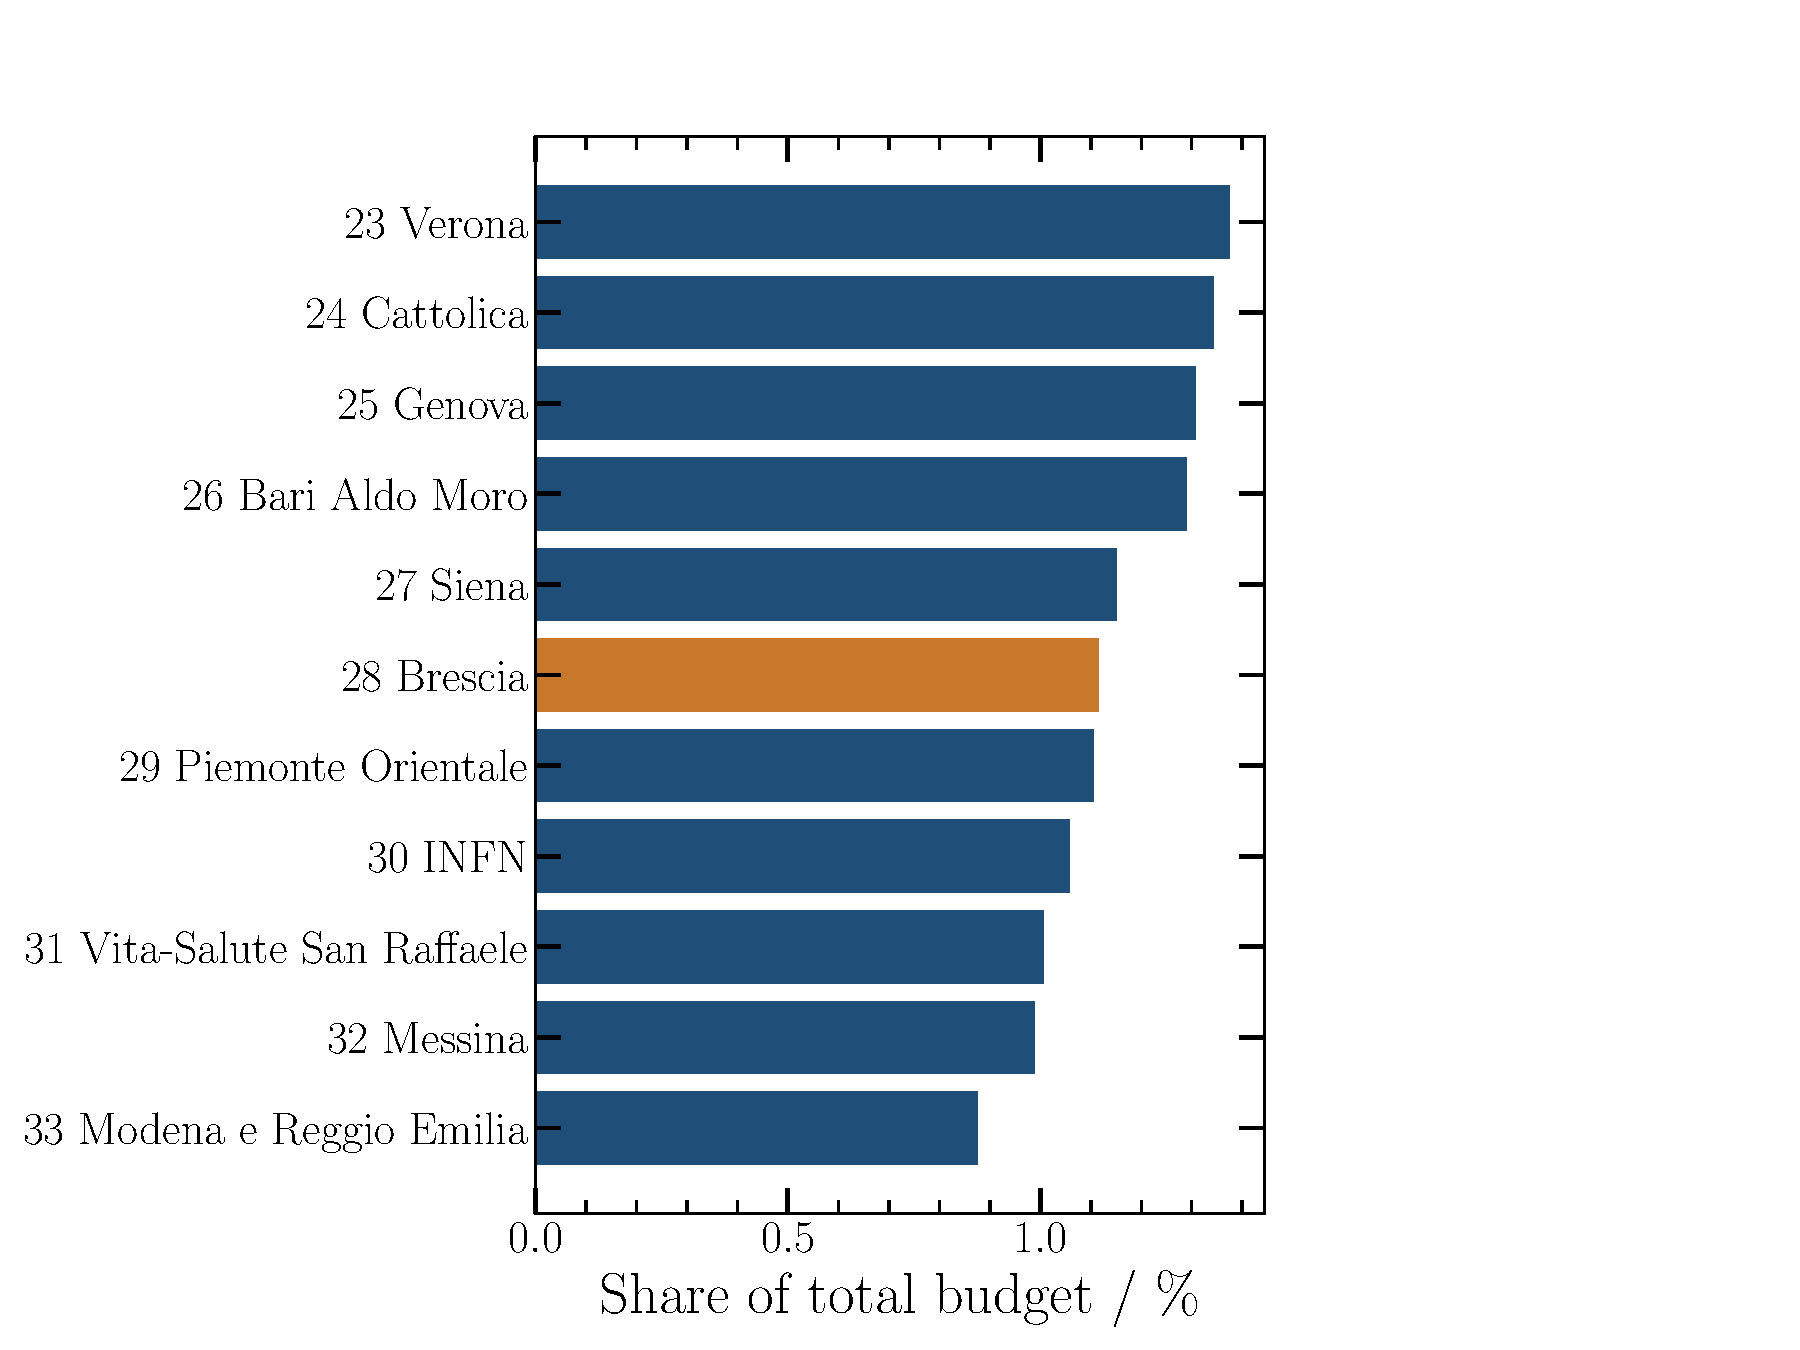
\includegraphics[width=0.65\textwidth]{../prin_out/figures/fact_brescia_neighbours.pdf}
\caption{Share of the total budget of Brescia and of the institutions ranked just above and below it.}
\end{figure}
\begin{figure}[H]
\centering
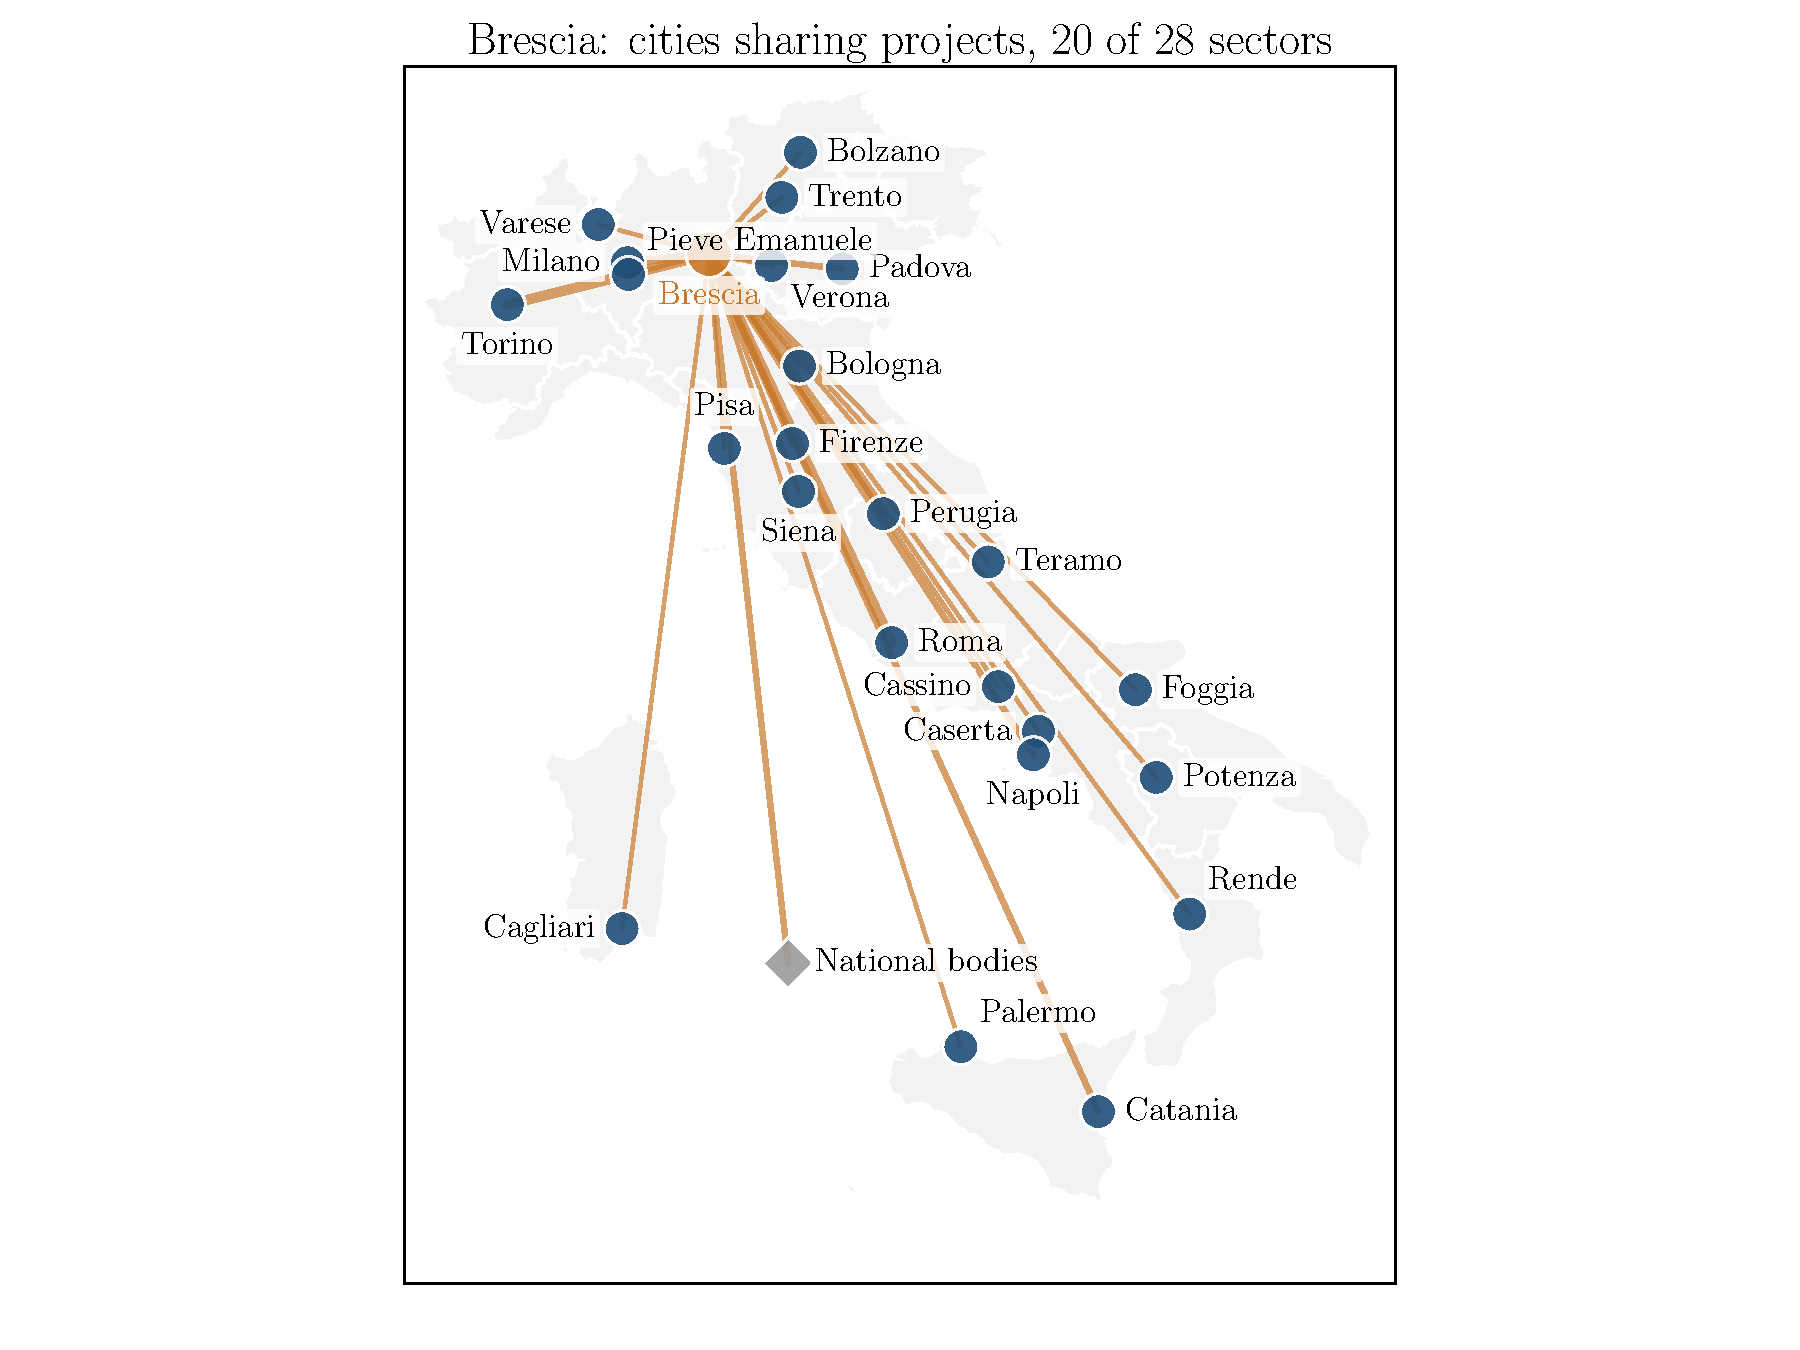
\includegraphics[width=0.75\textwidth]{../prin_out/figures/fact_brescia_map.pdf}
\caption{Cities sharing funded projects with Brescia (line width proportional to the number of projects).}
\end{figure}

\clearpage
\section{Institution fact sheet: Bolzano}
\textbf{Purpose.} To collect the figures of one institution and compare them with the other institutions of the same type.

\textbf{Result.} Bolzano received 0.34~M~EUR (0.16\% of the budget) in 2 projects, 0 as coordinator and 2 as partner, in 2 sectors; it ranks 73 of 91 institutions and 53 of 61 within its type.

\begin{table}[H]
\centering
\begin{tabular}{llr}
\toprule
Bolzano & Value & Median, public univ. \\
\midrule
Funding & 0.34~M~EUR, 0.16\% of the budget & 0.76\% \\
Rank & 73 of 91; 53 of 61 in its type &  \\
Funded projects & 2 & 8 \\
Sectors with a funded unit & 2 of 24 & 7 \\
Money received as PI & 0\% & 21\% \\
\bottomrule
\end{tabular}
\end{table}
{\footnotesize
\begin{longtable}{lllrp{4.2cm}p{2cm}p{3.2cm}}
\toprule
Sector & Role & Level & k EUR & Project & Coordinator & Other institutions \\
\midrule
\endhead
PE5 & RU & PO & 173 & TWIST — ToWard chiral light from Inverted Singlet-Triplet... & Padova & Basilicata, Brescia, Siena, Torino \\
PE6 & RU & PA & 171 & Embodied eXPERtise Transfer through Mutual Interpretation... & Verona & Catania, Federico II, Padova, Sapienza \\
\midrule
Total &  &  & 344 &  &  &  \\
\bottomrule
\multicolumn{7}{l}{\footnotesize Level of the leader: PO, PA, RTD, RU; n.a.: not a university leader or not found.} \\
\end{longtable}
}
\begin{figure}[H]
\centering
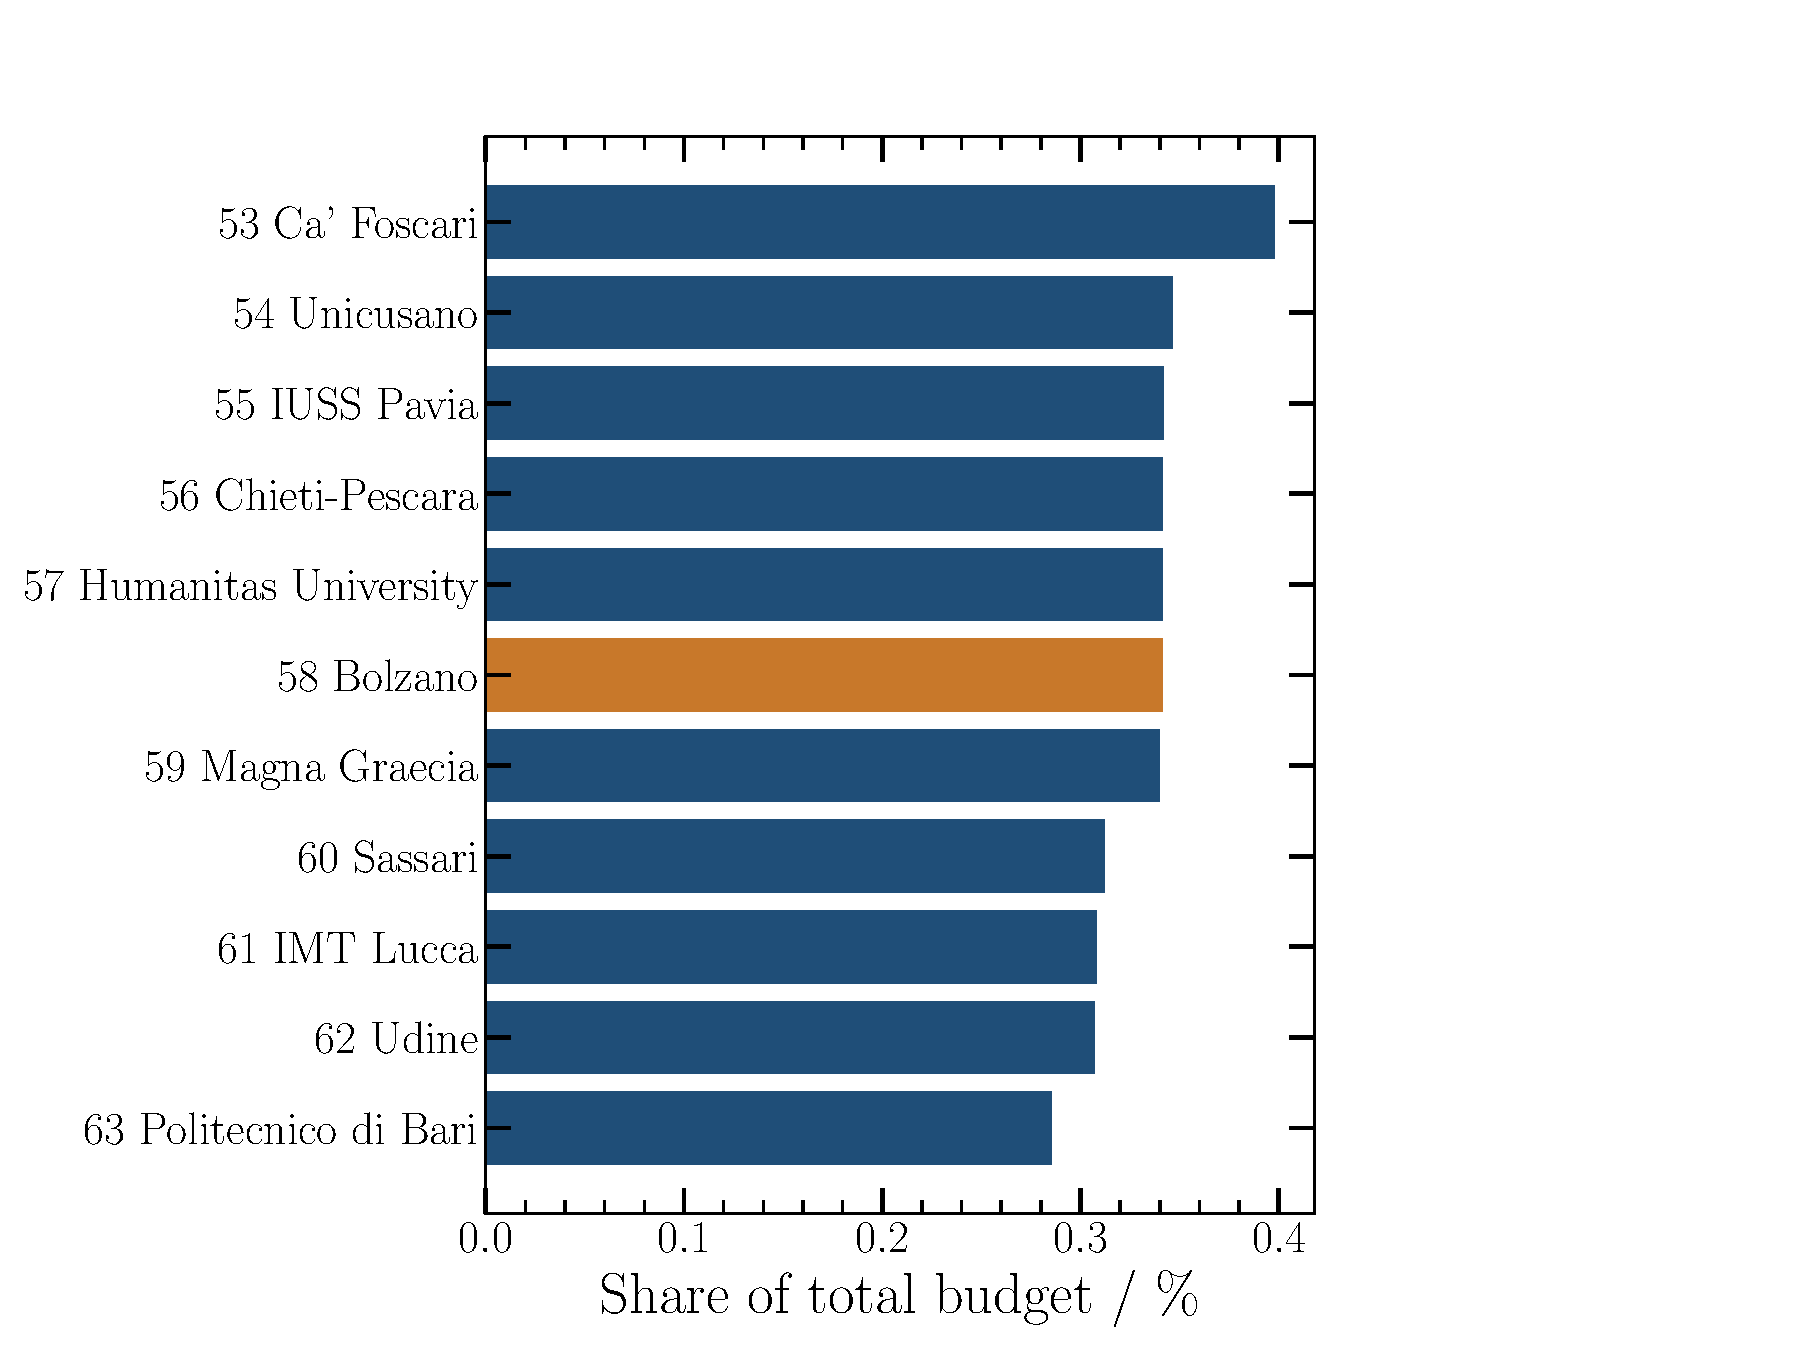
\includegraphics[width=0.65\textwidth]{../prin_out/figures/fact_bolzano_neighbours.pdf}
\caption{Share of the total budget of Bolzano and of the institutions ranked just above and below it.}
\end{figure}
\begin{figure}[H]
\centering
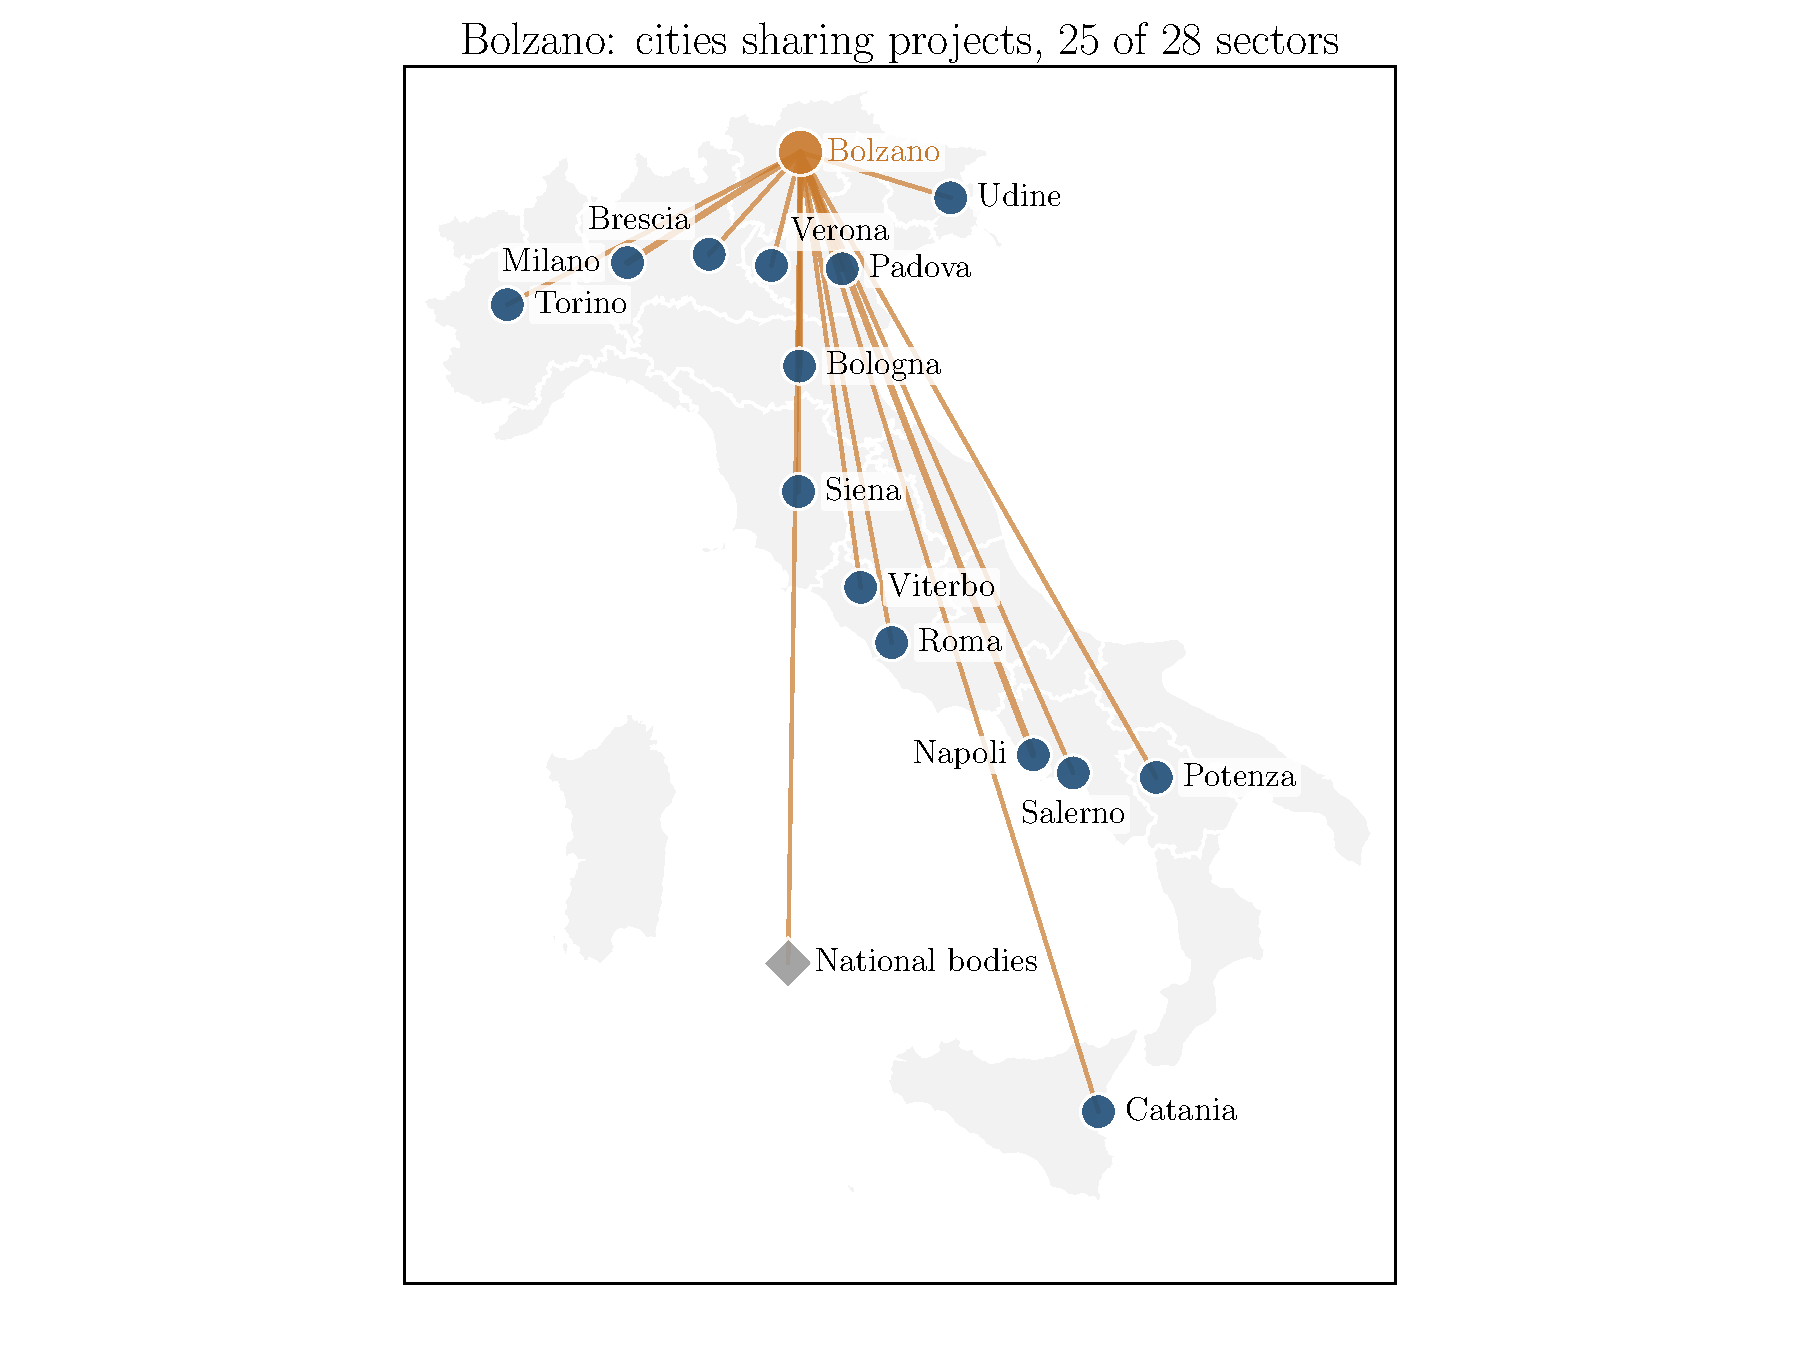
\includegraphics[width=0.75\textwidth]{../prin_out/figures/fact_bolzano_map.pdf}
\caption{Cities sharing funded projects with Bolzano (line width proportional to the number of projects).}
\end{figure}

\clearpage
\section{Institution fact sheet: Torino}
\textbf{Purpose.} To collect the figures of one institution and compare them with the other institutions of the same type.

\textbf{Result.} Torino received 9.41~M~EUR (4.37\% of the budget) in 42 projects, 8 as coordinator and 34 as partner, in 20 sectors; it ranks 3 of 91 institutions and 2 of 61 within its type.

\begin{table}[H]
\centering
\begin{tabular}{llr}
\toprule
Torino & Value & Median, public univ. \\
\midrule
Funding & 9.41~M~EUR, 4.37\% of the budget & 0.76\% \\
Rank & 3 of 91; 2 of 61 in its type &  \\
Funded projects & 42 & 8 \\
Sectors with a funded unit & 20 of 24 & 7 \\
Money received as PI & 27\% & 21\% \\
\bottomrule
\end{tabular}
\end{table}
{\footnotesize
\begin{longtable}{lllrp{4.2cm}p{2cm}p{3.2cm}}
\toprule
Sector & Role & Level & k EUR & Project & Coordinator & Other institutions \\
\midrule
\endhead
LS2 & RU & PA & 200 & Omics Signatures and Phenotypic Expression in... & Vanvitelli & Federico II, Genova \\
LS2 & RU & PO & 240 & Decoding and Targeting Cancer Plasticity & Vita-Salute San Raffaele & Brescia, Palermo, Trento \\
LS3 & RU & PO & 290 & The conventional and unconventional roles of the... & Milano Statale & Bologna, Padova \\
LS4 & RU & PO & 165 & Mechanisms and Outcomes of Metabolic Health in pituitary... & Federico II & Cattolica, Genova, Messina, Vita-Salute San Raffaele \\
LS4 & RU & PO & 150 & Multidimensional Analysis of Tumor Resistance and... & Federico II & CNR, Sapienza, Trento, Vanvitelli \\
LS4 & RU & PA & 167 & PRISM-T2D BCAA-Klotho-FGF23 Axis as a Multidirectional... & Milano-Bicocca & Campus Bio-Medico, Pisa, Sapienza, Vita-Salute San Raffaele \\
LS6 & RU & PO & 278 & Uncovering novel innate immune circuits governing... & Pavia & Humanitas University, Verona \\
LS7 & PI & PO & 521 & RISK-IT: Risk Miscalibration as a Fundamental Mechanism of... & this institution & Cagliari, Pisa, Sapienza \\
LS7 & RU & PO & 269 & Chemical EPigenomics of drug tolerant persister cells in... & Milano Statale & CNR, Sapienza \\
LS7 & RU & PO & 184 & Integrative Tumor and cfDNA Methylation Analysis to Predict... & Siena & Bari Aldo Moro, Federico II \\
LS8 & RU & n.a. & 174 & RESPOND - Integrated ecological and evolutionary responses... & Milano Statale & Padova, Tuscia \\
LS8 & RU & n.a. & 137 & Understanding the Functioning of Ecosystems emergiNg after... & Milano Statale & CNR, Tuscia \\
PE1 & RU & PO & 195 & Variational Methods, Geometric Analysis and Free Boundary... & Normale & Politecnico di Milano, Sapienza, Tor Vergata, Trento \\
PE1 & RU & PA & 205 & The interplay of geometry and topology in the study of... & Bologna & Pisa, Sapienza \\
PE10 & PI & PO & 249 & Mélanges Across Scales: Revealing the Rheological... & this institution & CNR, Genova, Modena e Reggio Emilia, Pisa \\
PE10 & RU & PO & 259 & The dawn of the Humboldt Current System: Paleogene origins,... & Pisa & Camerino, Milano-Bicocca \\
PE10 & RU & PO & 193 & A Multidisciplinary AppROach to unravel the seismic cycle in... & Padova & Federico II, INGV, Milano-Bicocca \\
PE2 & RU & PO & 149 & Non-perturbative dynamics of fundamental interactions from... & Roma Tre & INFN, Milano-Bicocca, Pisa, Tor Vergata \\
PE2 & RU & PA & 196 & BeamOn: a high‑precision, low‑material beam monitor for... & Cagliari & INFN, Piemonte Orientale, Trieste \\
PE3 & RU & PO & 215 & PROTEUS: Physics of Cancer Dynamics: Single Cells,... & Milano Statale & Padova, Sapienza, Vita-Salute San Raffaele \\
PE3 & RU & RTD & 127 & Quantum non-reciprocity (Q-NORE) & Milano-Bicocca & CNR, Ca' Foscari, Politecnico di Milano \\
PE4 & RU & n.a. & 265 & POC-PD: Graphene-Based Multisensor Bioelectronic Platforms... & CNR & Modena e Reggio Emilia, Parma \\
PE4 & RU & n.a. & 193 & PROcesses for green dimethyl Ether from sUstainable Sources... & Milano Statale & CNR, Pisa, Politecnico di Milano, Salerno \\
PE5 & PI & PA & 216 & Spatially Programmed 3D Adsorbents for Carbon dioxidE... & this institution & CNR, Milano Statale, Milano-Bicocca, Padova, Perugia \\
PE5 & RU & RTD & 173 & TWIST — ToWard chiral light from Inverted Singlet-Triplet... & Padova & Basilicata, Bolzano, Brescia, Siena \\
PE7 & PI & PO & 246 & DENDRA - Adaptive Dendritic Electronics for Self-Organizing... & this institution & CNR, Padova, Tor Vergata \\
PE9 & RU & PA & 157 & Unlocking the Full Cosmological Information of... & Milano Statale & Genova, INAF, SISSA, Trieste \\
SH3 & RU & n.a. & 240 & COBIKE - Co-Making Urban Cycling Infrastructures:... & Padova & CNR, Siena \\
SH3 & PI & n.a. & 334 & GREATWEALTH - Intergenerational equity and the Great Wealth... & this institution & IULM, Piemonte Orientale, Roma Tre, Siena \\
SH3 & RU & n.a. & 209 & "Beyond the Bystander". Preventing Gender-Based Violence in... & Modena e Reggio Emilia & Milano-Bicocca, Sapienza \\
SH4 & RU & RTD & 289 & Sensory evidence and PRIors in Nocebo Genesis (sPRINg) & Verona & Bologna, CNR \\
SH4 & RU & PA & 196 & Costs and Benefits of Acting Together: The Cognitive and... & Milano-Bicocca & Messina, Sapienza, Tor Vergata \\
SH5 & RU & RTD & 234 & Natural Intelligence: Ancient Perspectives on its Forms,... & Roma Tre & Bologna, Federico II, Firenze, Parma \\
SH5 & RU & RTD & 205 & Reconstructing the Hittite City: Text, Materiality, and... & Sapienza & CNR, Firenze, San Raffaele Roma \\
SH5 & RU & PA & 171 & ArchAut - An Archaeology of Italian Autofiction (1922-1975)... & Palermo & Messina, Roma Tre, Unicusano \\
SH6 & PI & PA & 366 & Beyond Institutions: Non-Institutional Economic Agency in... & this institution & CNR, Ca' Foscari, Pavia, Sapienza \\
SH6 & RU & PA & 213 & AFTER: Afterlives of fascism in everyday spaces & Siena & L'Aquila, Padova, Trento \\
SH6 & PI & PO & 259 & PatriarKeys. Patriarchy across the ages: Keys to decoding... & this institution & Genova, L'Orientale, Piemonte Orientale \\
SH7 & RU & PO & 243 & Circular Economy Data, Models and Indicators for Transition... & Ferrara & Milano-Bicocca, Molise, Parthenope, Roma Tre \\
SH8 & RU & n.a. & 130 & PASSIM Places And SoundS of Italian Musical life: Mapping,... & Milano Statale & Firenze, Link Campus University, Politecnico di Milano, Sapienza \\
SH8 & PI & n.a. & 308 & Metamorphic Matter. Reassessing Stucco and Plastic Materials... & this institution & Firenze, Internazionale UNINETTUNO, Trento, per Stranieri di SIENA \\
SH8 & RU & n.a. & 201 & C.A.R.M.A. – Crisis and Radical Medical Anthropology... & L'Orientale & Ca' Foscari, Palermo, Perugia \\
\midrule
Total &  &  & 9412 &  &  &  \\
\bottomrule
\multicolumn{7}{l}{\footnotesize Level of the leader: PO, PA, RTD, RU; n.a.: not a university leader or not found.} \\
\end{longtable}
}
\begin{figure}[H]
\centering
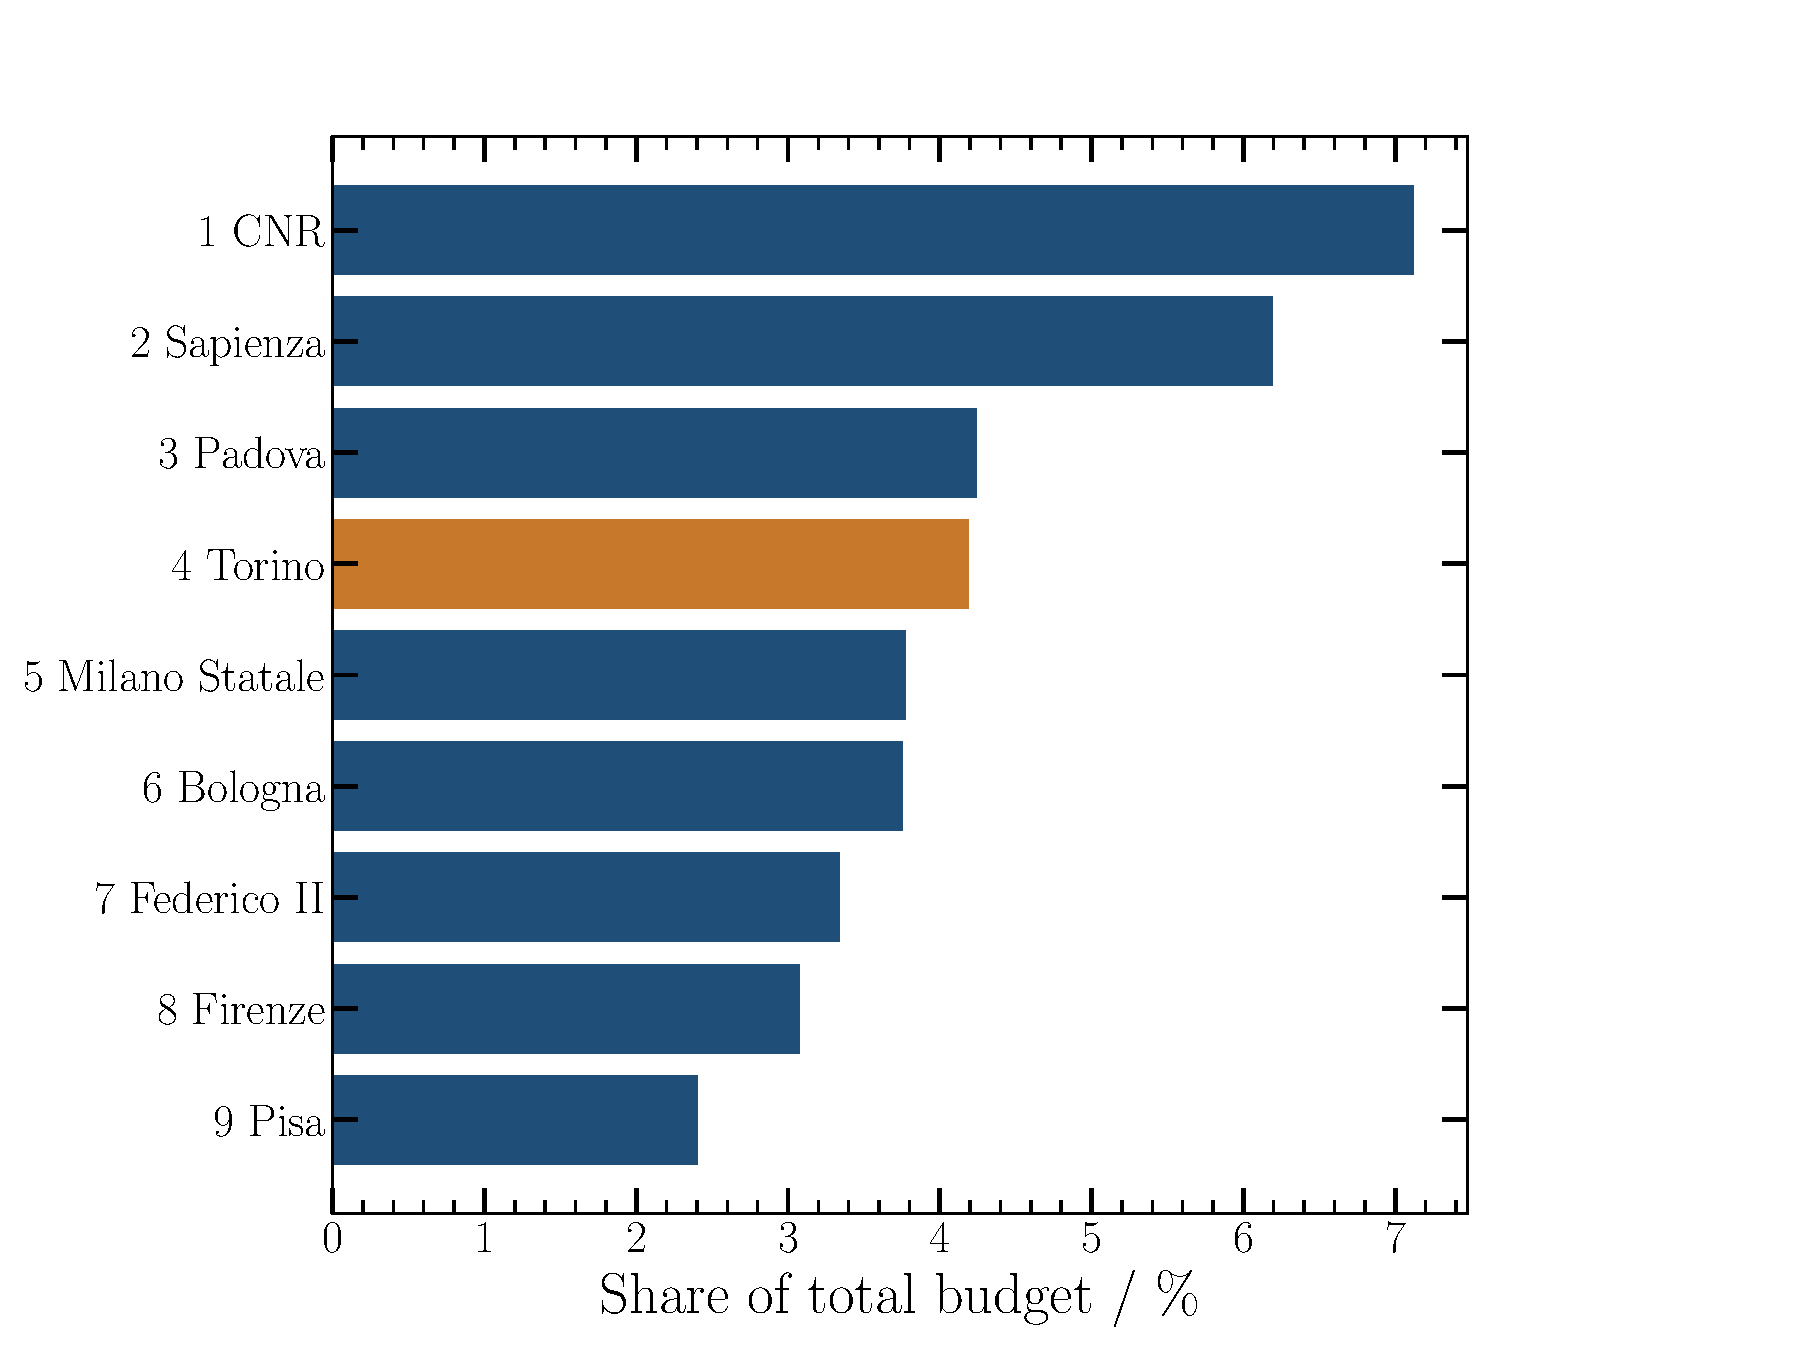
\includegraphics[width=0.65\textwidth]{../prin_out/figures/fact_torino_neighbours.pdf}
\caption{Share of the total budget of Torino and of the institutions ranked just above and below it.}
\end{figure}
\begin{figure}[H]
\centering
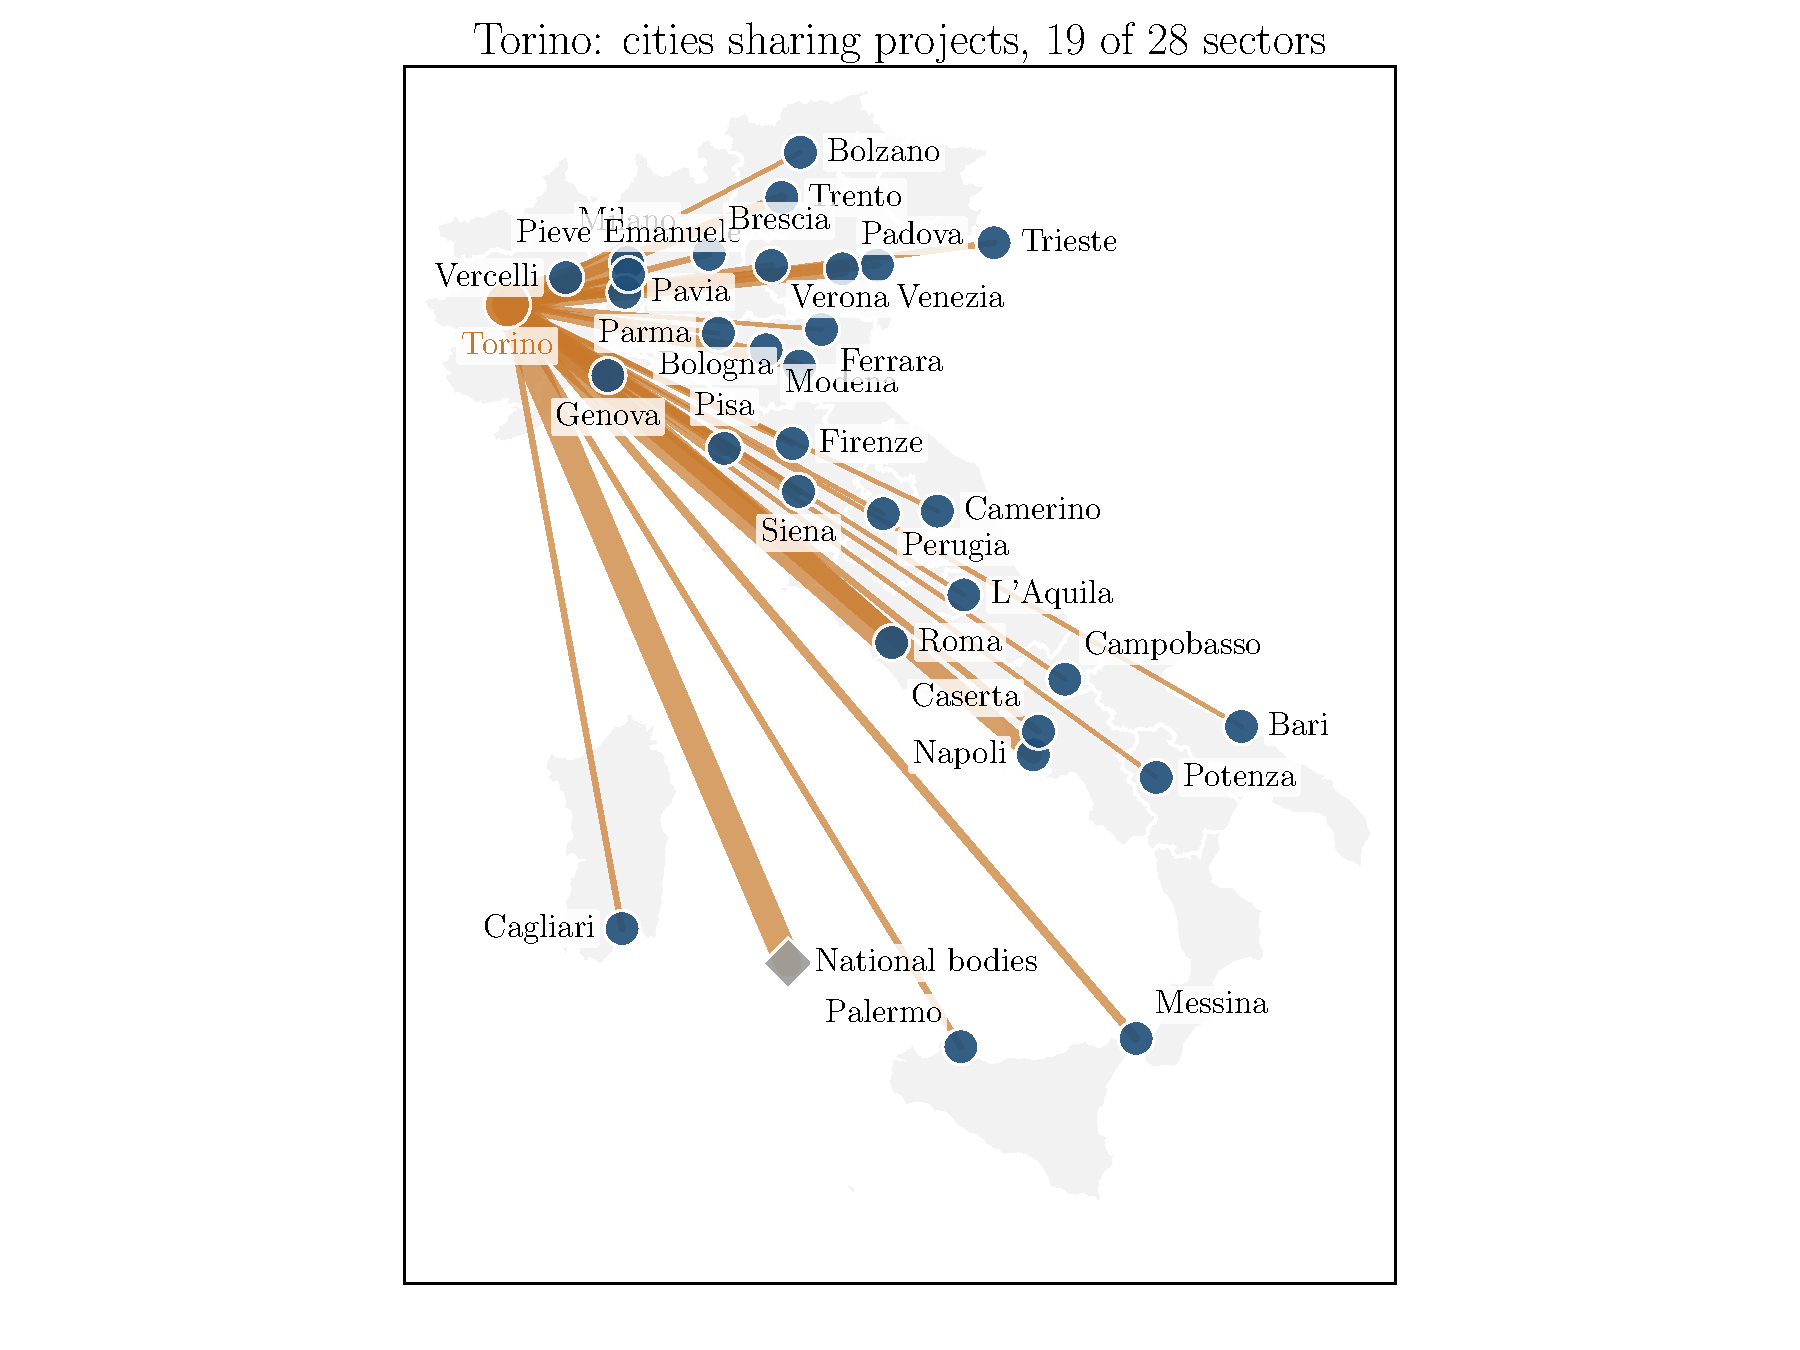
\includegraphics[width=0.75\textwidth]{../prin_out/figures/fact_torino_map.pdf}
\caption{Cities sharing funded projects with Torino (line width proportional to the number of projects).}
\end{figure}

\end{document}
